\documentclass[10pt]{article}
\usepackage[a4paper,margin=1.55cm]{geometry}
\usepackage[T1]{fontenc}
\usepackage[english]{babel}
\usepackage{lmodern}
\usepackage{microtype}
\usepackage{graphicx}
\usepackage{booktabs}
\usepackage{tabularx}
\usepackage{amsmath}
\usepackage{xcolor}
\usepackage[hidelinks]{hyperref}
\usepackage{caption}
\captionsetup{font=small,labelfont=bf}
\setlength{\parskip}{3pt}
\graphicspath{{../research/timecourse/figures/}{../research/person/figures/}{../research/revision/figures/}}
\definecolor{boxline}{HTML}{2a78d6}
\definecolor{boxbg}{HTML}{f7f9fc}
\newcommand{\questionbox}[1]{\par\smallskip\noindent\fcolorbox{boxline}{boxbg}{%
\parbox{\dimexpr\linewidth-2\fboxsep-2\fboxrule\relax}{#1}}\par\smallskip}

\title{Physiological Characterization and Detection Audit of Acute Stress in 314 People: Temporal Dynamics, Cardiac Morphology, Cortical Spatialization, Brain--Heart Coupling, and Appraisal at Fixed Stimulus}
\author{Team 12: Mathias Chebbah, Aurélien Saint-Grégoire, Ashley Russo\\
\small HABS Neuro-AI Hackathon, Université Paris-Saclay, November 2026}
\date{}

\begin{document}
\maketitle

\begin{abstract}
\noindent Characterizing an acute stress reaction physiologically---which systems change, in what order, with what cortical spatialization, and under which autonomic branch---and rigorously auditing the validity of multimodal detectors are two core problems in affective neuroscience and non-verbal physiological monitoring (from neurofeedback and lab studies to non-communicating populations: acute pain assessment in pre-verbal pediatrics, locked-in syndrome, coma, and general anesthesia). Using the multimodal HABS dataset (314 healthy volunteers, 22,974 trials across 252 ten-second clips, 64-channel EEG, ECG, skin conductance, and respiration), we conduct a comprehensive physiological characterization and methodological audit.
\textbf{(1)~Criterion and raw emotions:} audited against non-circular rank-1 self-reported emotions (cohorts~2--5, $n = 3,938$ included trials), our composite criterion (\emph{valence $\le 4$ and arousal $\ge 6$}) achieves 89.2\% negative purity at rank~1 (97.2\% across ranks~1--3; 72.5\% core acute threat; 5.3\% incoherent labels). Tightening to $2/8$ raises purity to 95.3\% and doubles skin ($d = +0.14 \to +0.34$) and EEG delta ($+0.13 \to +0.30$) effects while halving cardiac deceleration ($-0.11 \to -0.04$) via antagonistic sympathetic recruitment; $3/7$ maximizes detection (AUC 0.549). Direct emotion analysis separates fear (heart $-0.20$, skin $+0.25$, resp.\ $-0.11$, alpha $-0.12$), disgust (heart $-0.20$, delta $+0.15$), and sadness (flat across sensors), while unsupervised clustering fails to recover affective states ($\mathrm{ARI} < 0.009$).
\textbf{(2)~ECG morphology and rich EEG dynamics:} after auto-correcting inverted ECG polarity in 96.6\% of trials, RR lengthens ($+5.1$~ms, $d = +0.116$) while PR interval and PR segment (AV-node conduction) are strictly null ($d = -0.005$ to $+0.010$) and the apparent Bazett QTc drop ($-0.092$) vanishes after controlling $\Delta\mathrm{RR}$ ($-0.007$), establishing fast vagal sinus braking rather than adrenergic AV acceleration. Early EEG temporal volatility (1-s delta max jump $+0.151$) and biphasic spatial reorganization (early homogenization followed by post-clip focalization, alpha spatial entropy $-0.076$) substantially enrich the cortical signature.
\textbf{(3)~Raw brain--heart control:} unprocessed \texttt{CURATED} EEG (62-channel CAR, no ICA, identical R peaks) replicates the null primary heartbeat-evoked potential (HEP: $d = +0.038$ raw vs.\ $+0.039$ ICA; ICA-removed difference $+0.012$).
\textbf{(4)~Fixed-video appraisal and sensitivity:} excluding borderline trials to contrast stressed against genuinely calm viewers watching the \emph{exact same} video raises same-video AUC from 0.525 to 0.564 (heart 0.553, delta 0.564, skin $d = +0.197$). In the $2\times 2$ Consensus $\times$ Appraisal matrix, calm viewers of high-consensus stressful clips show zero bradycardia ($-0.49$~bpm) and zero skin-conductance rise ($+0.014\,\mu$S), leaving only occipital alpha desynchronization automatic ($-0.33$ to $-0.41$). Trial-level individual sensitivity tracks prefrontal $\beta/\gamma$ ($-0.035$ to $-0.039$) and centroparietal delta (93\% intact after pre-ICA Fp1/Fp2 ocular control), while trait sensitivity tracks resting heart rate ($r = +0.140$) and pre-stimulus gamma ($+0.165$).
\textbf{(5)~Four-phase and sequence detection:} on a fresh person $\times$ theme split, replacing 1-s bins with 4 enriched phases and sequence convolutions lifts double-unseen sealed-test AUC from 0.526 to 0.589 (linear enriched) and 0.586 (continuous valence--arousal Ridge, best overall: dev 0.576, unseen themes 0.558, unseen people 0.607, 0.656 vs.\ relaxed), whereas ECG P-QRS-T intervals and nonlinear MLP/GBDT heads do not improve unseen-stimulus generalization.
\end{abstract}

\section{Introduction and Neuroscientific Framing}

\paragraph{Why characterize acute stress and audit physiological detectors?}
An acute stress reaction coordinates the central nervous system with both branches of the autonomic nervous system (vagal parasympathetic and sympathetic adrenergic/sudomotor). Two foundational scientific questions---independent of any single occupational scenario---motivate this study:
\begin{enumerate}
\item \textbf{Descriptive neurophysiology:} during a brief acute stress reaction, which central and peripheral signals actually change, in what temporal order, with what scalp spatialization and homogeneity, and under the control of which autonomic branch (vagal orienting braking vs.\ sympathetic adrenergic drive)?
\item \textbf{Methodological audit of detectors:} how accurately can a multimodal setup detect acute stress in an unseen person facing an unseen situation, and what is it actually reading---a stereotyped sensory reflex imposed by the stimulus, or the individual's own subjective appraisal?
\end{enumerate}

This dual inquiry underpins physiological acute-stress monitoring across a wide spectrum of contexts: closed-loop labeling for neurofeedback, standard affective-neuroscience paradigms, and critically clinical populations where patients \emph{cannot self-report verbally}. From acute pain estimation in pre-verbal pediatric patients (acute pain being a potent driver of acute stress) to locked-in syndrome, disorders of consciousness (coma), and assessing nociceptive or stress-pathway activation under general anesthesia, the clinical validity of any non-verbal biomarker depends on separating genuine internal distress from an automatic sensory orienting reflex.

\paragraph{Scope and structural limits of HABS.}
The HABS dataset brings together 314 healthy volunteers (22,974 audited trials across 252 ten-second audiovisual clips) recorded concurrently with 64-channel EEG, ECG, skin conductance (EDA/GSR), and a respiration belt. Eye tracking was excluded per organizer advice due to temporal desynchronization. HABS contains no error-generating cognitive task, no cortisol, and no somatic pain; its unique strength is scale (314 people vs.\ 15--50 in most laboratory studies \cite{palomba2000,hagenaars2014,schubring2019}) combined with a crossed design where every video was watched by 13 to 234 different people (median 83), allowing clean separation of stimulus consensus from individual appraisal. Moreover, recent work by the HABS team demonstrated that EEG emotion classifiers can score high merely by identifying the stimulus rather than the affective state \cite{gerster2026}, echoing earlier caveats in video-watching stress detection \cite{giannakakis2015}.

Earlier phases of this project (Studies 04--06) established a baseline 1-s time course, modest detection, a null heartbeat-evoked potential (HEP), and an apparent dominance of video consensus over individual ratings. A rigorous clinical and neuroscientific critique raised six substantive challenges: (i)~auditing and purifying the valence--arousal stress criterion against raw reported emotions; (ii)~benchmarking direct classifiers on frequent rank-1 emotions and exploring unsupervised structure; (iii)~moving beyond noisy 1-s bins to four physiological phases, beat-by-beat ECG P-QRS-T delineation (specifically PR interval/segment indexing adrenergic AV-node conduction), EEG temporal variation and spatial homogeneity, and sequence-aware architectures exploiting $t \to t+1$ dependence; (iv)~testing whether ICA preprocessing destroyed cardiac-covariant cortical activity in the HEP analysis; (v)~avoiding reductive ``person vs.\ situation'' terminology, auditing per-video class imbalance and borderline dilution in fixed-video controls, and testing an all-or-nothing (on/off) appraisal profile; and (vi)~mapping EEG topography of stress sensitivity in light of anxiety disorders. This paper answers all six challenges empirically under a protocol frozen prior to computation (\texttt{journal/07\_comprehensive\_revision.md}).

\questionbox{\textbf{Six research questions structuring this study.}
\begin{description}
\item[Q1 -- Criterion \& raw emotions:] Does the valence--arousal criterion genuinely capture acute stress, how do purity and physiological effects evolve under threshold tightening, and how do direct rank-1 emotion classifiers and unsupervised clustering behave?
\item[Q2 -- 4-phase dynamics, ECG morphology \& EEG spatialization:] In what order do signals move, does P-QRS-T morphology (PR segment, QRS, QT/QTc, T wave) reveal early adrenergic modulation, and what do EEG temporal volatility and spatial homogeneity add?
\item[Q3 -- Brain--heart coupling \& preprocessing:] Does the heartbeat-evoked potential (HEP) shift under acute stress, and did ICA preprocessing remove cardiac-covariant cortical signal relative to unprocessed \texttt{CURATED} EEG?
\item[Q4 -- Normative consensus vs.\ fixed-video appraisal:] Once per-video skew, borderline trials, and single-axis valence/arousal effects are controlled, does physiology respond automatically to the stimulus or only when appraised as stressful (threshold / on--off mechanism)?
\item[Q5 -- EEG topography of stress sensitivity:] Which bands and cortical regions track trial-level idiosyncratic sensitivity and between-subject trait sensitivity, and does centroparietal delta survive a pre-ICA ocular proxy control?
\item[Q6 -- Multi-scale detection \& sequence architectures:] Do enriched 4-phase features, $\Delta(t\to t+1)$ transitions, P-QRS-T waves, EEG spatial/temporal dynamics, and sequence-aware or nonlinear models improve unseen-person and unseen-theme generalization?
\end{description}}

\section{Detailed Methods}

To make every analytical choice transparent and reproducible, we detail the data structure, signal processing, and statistical inference below.

\subsection{Dataset, Hardware Acquisition, and HABS Preprocessing}
We include all 22,974 audited trials (314 participants, 5 cohorts, 508 recordings, 252 videos spanning 84 themes) whose BDF triggers match metadata timestamps within 25~ms. In this released \texttt{labels\_train.csv}, \texttt{flagged\_outliers} equals 0 on 100\% of retained trials (flagged trials having been removed upstream). Cohorts~2--5 ($n = 17,142$, 209 people) provide continuous 1--9 valence/arousal ratings and 1--3 participant-selected emotions from 12 categories (\texttt{self\_reported\_emotion\_1..3}); cohort~1 ($n = 5,832$, 105 people) provides integer ratings without discrete emotion choices.

Recordings (1,000~Hz, ANT Neuro eego~64 + SenseBox) comprise: (i)~64-channel 10--10 EEG (online Cz/CPz reference); (ii)~a \textbf{single bipolar ECG lead} (two Ag/AgCl electrodes placed bilaterally in the infraclavicular region, lead-I equivalent)---multi-lead spatial ECG comparison is therefore not possible in HABS; (iii)~skin conductance on the non-dominant hand (converted to $\mu$S via the vendor calibration curve without silent clipping); and (iv)~a lower-thoracic piezoelectric respiration belt.

HABS's \texttt{PREPROCESSED} pipeline drops T9/T10, applies a 50-Hz notch filter to peripheral channels, zero-phase FIR filters EEG to 0.5--48~Hz, re-references to the 62-channel common average (CAR), and runs Picard ICA with \emph{ICLabel}, subtracting components with eye probability $\ge 0.75$ or muscle/line/channel probability $\ge 0.90$. Although ICLabel's ``heart'' class is not explicitly listed in those rejection criteria, cardiac-covariant cortical activity could still leak into rejected components---motivating our direct empirical test on raw \texttt{CURATED} files (Section~\ref{sec:meth_hep}).

\subsection{Criterion Audit, Raw Emotion Classifiers, and Unsupervised Analysis (Q1)}
\paragraph{Non-circular criterion audit.}
Because HABS's \texttt{final\_emotion\_label} is refined via kernel density estimation in the valence--arousal plane, validating a valence--arousal rule against it would be circular. We therefore audit exclusively against the participant's raw rank-1 choice (\texttt{self\_reported\_emotion\_1}, extended to ranks~2--3 in \texttt{criterion\_full}), available on 100\% of cohorts~2--5 ($n = 17,142$). The 12 categories are grouped into \emph{core acute threat} (anger, fear, disgust), \emph{non-threat negative} (sadness, guilt), \emph{surprise} (ambivalent, including aversive startle), and \emph{stress-incoherent} (joy, excitement, relaxation, sensuality, neutral, curiosity). We sweep ten thresholds---from the open quadrant ($V < 5 \cap A > 5$) to the extreme corner ($V \le 2 \cap A \ge 8$) plus three asymmetric cuts---tracking purity, per-emotion recall, physiological effect sizes, and detection AUC.

\paragraph{Supervised rank-1 emotion models and the theme-fold prior-shift trap.}
On cohorts~2--5 ($n = 17,142$), we run $3\times 3$ double-blocked cross-validation (people $\times$ themes) for: (i)~nine binary classifiers (one-vs-rest and one-vs-neutral) covering frequent emotions (\emph{fear, anger, disgust, sadness, joy, relaxation, neutral}), \emph{core threat}, and \emph{all negative}; and (ii)~a unified $(K+1) = 5$-class classifier (\emph{fear, anger, disgust, sadness, other}). Development revealed an instructive methodological pitfall: because video themes cluster by emotion, splitting themes into 3 folds produces unequal training base rates across folds. Without class balancing, logistic intercepts shift across theme folds and produce artificially sub-chance within-person AUCs (down to 0.387 for anger) once fold predictions are concatenated. Setting \texttt{class\_weight="balanced"} (or applying exact Bayes log-likelihood-ratio calibration $\log\frac{p}{1-p} - \log\frac{\pi_{\text{train}}}{1-\pi_{\text{train}}}$ to neural outputs) pins the training prior to 0.50 in every fold and eliminates this artifact with zero leakage.

\paragraph{Unsupervised exploration.}
On 36 within-person centered physiological features (heart, skin, respiration amplitude/rate in early/late phases, plus 6 regions $\times$ 5 EEG bands baseline-corrected), without exposing any labels, we apply PCA (10 components) followed by $k$-means ($k = 2$--$6$) and Gaussian mixture models (GMM, $k = 2$--$5$) on the top 8 PCs, measuring spontaneous alignment with stress, 5 emotion classes, theme, and video identity via adjusted Rand index (ARI) and normalized mutual information (NMI).

\subsection{1-s and 4-Phase Dynamics, ECG P-QRS-T Delineation, and Rich EEG Features (Q2)}
Complementing Study~05's 1-s extraction ($-3$ to $+12$~s), a new backend extractor (\texttt{decoding/\allowbreak rich\_extract.py}) ran on the HABS compute backend to extract 650 columns across all 22,974 trials organized into four physiological phases: \textbf{Reference} $[-3, 0)$~s, \textbf{Early} $[0, 5)$~s, \textbf{Late} $[5, 10)$~s, and \textbf{Post-exposure} $[10, 12)$~s, plus full-video $[0, 10)$~s for ECG morphology.

\paragraph{Beat-by-beat ECG P-QRS-T delineation and the polarity discovery.}
Direct inspection of raw recordings revealed that HABS's infraclavicular lead has \textbf{inverted polarity in 96.6\% of trials} (negative P and T waves, positive deep S wave), causing standard polarity auto-inversion in NeuroKit2 to fail (delineating only 2\% of T waves on the validation sample). We therefore built a per-recording template-guided delineator (\texttt{delineate\_ecg}): (1)~QRS detection (5--25~Hz) and median-beat template construction on $[-350, +550]$~ms; (2)~polarity alignment via joint vote of P ($[-240, -70]$~ms) and T ($[+130, +420]$~ms, upright in sinus lead~I), followed by positive R-peak refinement; (3)~artifact-beat rejection by QRS template correlation ($r < 0.70$, median clean-beat rate 99.2\%); and (4)~beat-by-beat fiducial localization (0.5--15~Hz for P/T, 1--35~Hz for QRS slopes) of $\mathrm{P}_{\text{on}}, \mathrm{P}_{\text{pk}}, \mathrm{P}_{\text{off}}, \mathrm{QRS}_{\text{on}}, \mathrm{R}, \mathrm{QRS}_{\text{off}}, \mathrm{T}_{\text{pk}}, \mathrm{T}_{\text{off}}$ within strict physiological bounds. Per phase we average HR, RR, RMSSD, \textbf{PR peak} ($\mathrm{R} - \mathrm{P}_{\text{pk}}$, noise-robust), \textbf{clinical PR interval} ($\mathrm{QRS}_{\text{on}} - \mathrm{P}_{\text{on}}$), \textbf{pure PR segment} ($\mathrm{QRS}_{\text{on}} - \mathrm{P}_{\text{off}}$, indexing AV-node delay), QRS width, QT, Bazett QTc ($\mathrm{QT}/\sqrt{\mathrm{RR}}$), Fridericia QTc ($\mathrm{QT}/\mathrm{RR}^{1/3}$), RT peak, and T/R amplitude ratio. To separate intrinsic dromotropic or repolarization effects from heart-rate coupling, every metric is also tested in a within-person regression adjusted for $\Delta\mathrm{RR}$.

\paragraph{EEG spatial homogeneity, temporal variation, and pre-ICA ocular proxy.}
For each phase and band ($\delta, \theta, \alpha, \beta, \gamma$), Welch PSD (1.5-s windows in reference, 2-s in early/late, 1-s in post) yields: (i)~6 regional log-powers; (ii)~four \textbf{spatial homogeneity} indices across all 62 channels---inter-channel SD (\texttt{sp\_std}), robust IQR (\texttt{sp\_iqr}), normalized Shannon spatial entropy of linear power (\texttt{sp\_ent} $\in [0, 1]$, 1 = uniform scalp power), and inter-region SD; (iii)~three gradients/asymmetries---anterior--posterior gradient (frontal $-$ occipital), frontal alpha/band asymmetry (\texttt{FAA}), and temporal asymmetry; and (iv)~three \textbf{within-phase temporal variation} features from 1-s sub-windows---temporal SD (\texttt{tvar}), linear slope (\texttt{tslope}), and maximum adjacent 1-s jump $|\Delta_t|$ (\texttt{maxjump}). Explicit phase transitions $\Delta(t\to t+1)$ (0 at reference, $\text{early}-\text{ref}$, $\text{late}-\text{early}$, $\text{post}-\text{late}$) expose sequential structure directly. Finally, from unprocessed \texttt{CURATED} EEG we extract frontopolar peak-to-peak amplitude (Fp1/Fp2, $[0, 2]$~s) as a direct pre-ICA blink/startle proxy to test whether early delta reflects ocular leakage.

\subsection{Brain--Heart Coupling: Direct \texttt{CURATED} Raw vs.\ \texttt{PREPROCESSED} ICA Test (Q3)}
\label{sec:meth_hep}
To test whether \texttt{PREPROCESSED} ICA suppressed cardiac-covariant cortical activity, we extracted the HEP directly from \textbf{raw unprocessed \texttt{CURATED}} recordings with \textbf{no ICA}: dropping T9/T10 for an identical 62-channel CAR montage, 0.5--30~Hz bandpass filtering, epoching around the \textbf{exact same refined R peaks} as \texttt{hep\_extract.py} ($-200$ to $+600$~ms in sixteen 50-ms bins, $-200$ to $-50$~ms baseline), and rejecting epochs at both the standard 100\,$\mu$V and relaxed 200\,$\mu$V thresholds. Trial-by-trial pairing of \texttt{CURATED} and \texttt{PREPROCESSED} yields the exact \emph{ICA-removed waveform} ($\mathrm{HEP}_{\text{raw}} - \mathrm{HEP}_{\text{ICA}}$) locked to each heartbeat. The pre-specified primary window is 250--600~ms across frontal and central regions, analyzed before and after within-person adjustment for cardiac field amplitude (ECG in the same window) and mean RR \cite{parkblanke2019}.

\subsection{Normative Consensus, Fixed-Video Appraisal, \texorpdfstring{$2\times 2$}{2x2} Matrix, and EEG Sensitivity (Q4--Q5)}
\paragraph{Conceptual reframing and decomposition.}
Rather than reductive ``person vs.\ situation'' labels, we separate: (1)~the \textbf{normative / consensus component} (\emph{shared part}), estimated for trial $(p, v)$ as the leave-one-out mean of other viewers' centered ratings of video $v$ ($\ge 9$ other viewers), capturing both sensory stimulus properties and highly reproducible stereotypical human reactions; and (2)~the \textbf{idiosyncratic component} (\emph{own part}), viewer $p$'s residual from video $v$'s consensus, capturing individual sensitivity to that clip.

\paragraph{Non-adjacent fixed-video contrasts and $2\times 2$ matrix.}
High-consensus stressful videos suffer severe class imbalance, and the ``not stressed'' complement mixes genuinely calm viewers with borderline viewers (e.g., $V = 3.5, A = 5.5$). We first audit the per-video stress-rate histogram across all 252 clips, then evaluate at strictly fixed video: (i)~polarizing clips only ($0.20 \le p_v \le 0.80$, pair-weighted and unweighted video-level AUC); (ii)~\textbf{non-adjacent ``stressed vs.\ calm''} contrasts within the \emph{same} video ($V \le 4, A \ge 6$ vs.\ $V \ge 5, A \le 5$, and strict $V \ge 5.5, A \le 4.5$), reporting both AUC and within-video Cohen's $d$; and (iii)~single-axis pure contrasts (pure valence $V \le 3.5$ vs.\ $\ge 5.5$ at $A \ge 5$; pure arousal $A \ge 6.5$ vs.\ $\le 4$ at $V \le 4.5$).

To separate automatic stimulus reflexes from threshold/on--off appraisal, we build the \textbf{$2\times 2$ Stimulus Consensus $\times$ Viewer State matrix} crossing three consensus strata (\emph{low} $p_{v,-i} \le 10\%$, \emph{polarizing} 20--55\%, \emph{high} $\ge 50\%$) against three viewer states (\emph{very calm}, \emph{borderline}, \emph{stressed}). Within participants, we test: (a)~\emph{pure stimulus effect in calm viewers} (high- vs.\ low-consensus video while viewer remains calm); and (b)~\emph{pure appraisal effect at fixed video stratum} (stressed vs.\ calm on clips of matched consensus). We also plot 8-bin person-centered dose--response curves across valence, arousal, and consensus.

\paragraph{Trial-level and trait-level EEG sensitivity topography.}
We map $\beta_{\text{own}}$ across all 6 regions $\times$ 5 bands, frontal asymmetry (FAA), and all 62 electrodes. Between participants ($N = 314$), \textbf{trait stress sensitivity} is defined as each person's mean stress-rating bias relative to peers watching the \emph{same} videos ($\overline{s_{p,v} - p_{v,-p}}$, adjusted for cohort) and correlated with pre-stimulus ($[-3, 0]$~s) EEG topography, resting HR, and average phasic physiological reactivity.

\subsection{Detection Protocol, Sequence Architectures, and Inference (Q6)}
All predictive models are evaluated on a fresh deterministic person $\times$ theme split (\texttt{SALT =} \texttt{habs-\allowbreak revision-\allowbreak 2026-\allowbreak 11-\allowbreak 23}) ensuring zero person or theme leakage ($3\times 3$ CV on development; sealed tests opened once on unseen people, unseen themes, and unseen both). We benchmark twelve configurations: 1-s baseline, 4 phases, progressive ablations adding $\Delta(t\to t+1)$ transitions, ECG P-QRS-T waves, EEG spatial homogeneity, and EEG temporal variation, continuous valence--arousal Ridge, \emph{HistGradientBoosting}, and explicit sequence architectures (48 multi-scale 1D convolutional filters over the 12-s multivariate series plus first/second temporal derivatives and lag-1 persistence, paired with linear and Bayes-calibrated MLP heads). All 95\% CIs use 2,000 person-level (or video-level) bootstrap resamples \cite{varoquaux2018}.

\section{Results}

\subsection{Stress Criterion Audit, Purification, and Discrete Emotions (Q1)}

\paragraph{Sanity check against raw self-reported emotions.}
Across all 3,938 trials included in our standard criterion ($V \le 4 \cap A \ge 6$) with raw emotion labels (cohorts~2--5, 100\% coverage), rank-1 emotion counts strongly validate the rule (Figure~\ref{fig:criterion}A): \textbf{anger} (25.7\%), \textbf{fear} (23.9\%), \textbf{disgust} (22.9\%), and \textbf{sadness} (14.9\%) dominate overwhelmingly, followed by \emph{surprise} (5.5\%, mostly aversive startle), curiosity (2.7\%), guilt (1.8\%), neutral (1.4\%), and excitement (1.1\%), while relaxation (0.13\%), sensuality (0.03\%), and joy (0.03\%) are essentially absent. Overall, \textbf{89.2\% report a negative emotion at rank~1} (72.5\% core acute threat: anger, fear, disgust), and \textbf{97.2\% report a negative emotion in ranks~1--3} (90.1\% core threat). Even among the rare 5.3\% ($n = 209$) incoherent rank-1 trials, 69.9\% report a negative emotion at rank~2 or~3 (and 77.3\% of rank-1 \emph{surprise} trials do). The criterion captures 69.7\% of all anger, 66.2\% of all fear, and 49.6\% of all disgust while rejecting 99.9\% of joy, 99.7\% of relaxation, and 97.7\% of neutral trials.

\begin{figure}[t]
\centering
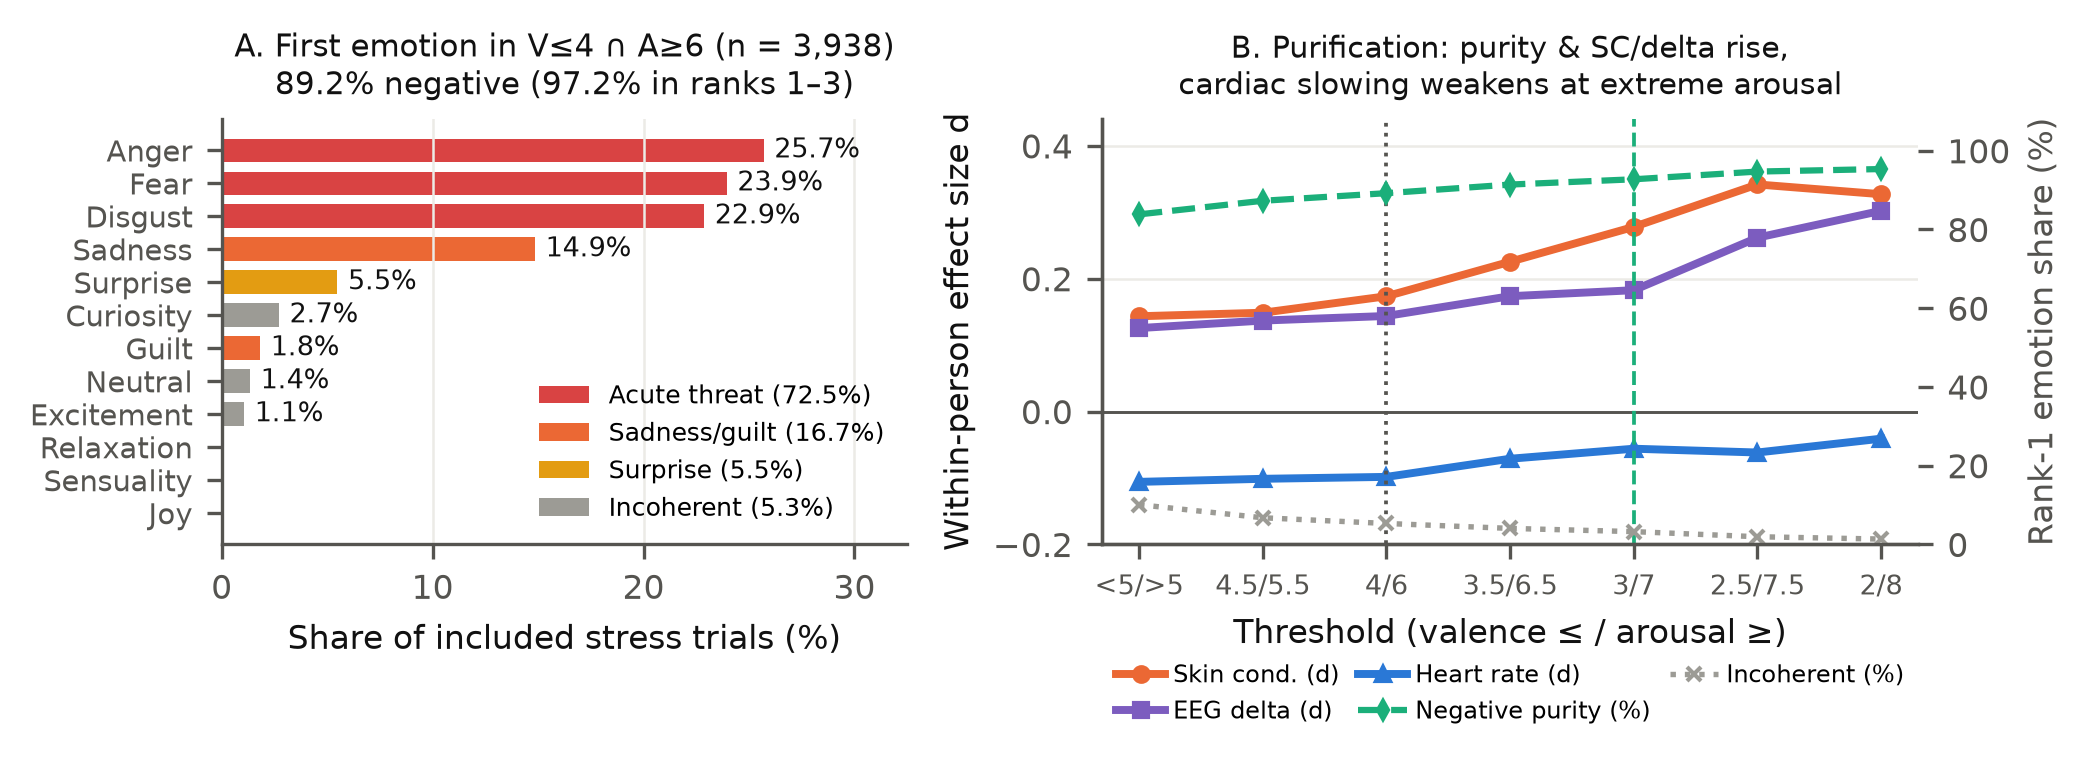
\includegraphics[width=\linewidth]{fig1_criterion.png}
\caption{\textbf{Stress criterion audit and purification sweep (Q1).} \textbf{A.} Rank-ordered raw rank-1 emotion (\texttt{self\_reported\_emotion\_1}, non-circular) inside $V \le 4 \cap A \ge 6$ (cohorts~2--5, $n = 3,938$). \textbf{B.} Sweep across 7 symmetric thresholds: negative purity rises from 83.8\% to 95.3\% and incoherent labels fall from 10.1\% to 1.4\%; skin and delta effects double while cardiac deceleration weakens at extreme arousal.}
\label{fig:criterion}
\end{figure}

\paragraph{Purification curve and unexpected autonomic divergence.}
Sweeping thresholds (Figure~\ref{fig:criterion}B, Table~\ref{tab:purification}) uncovers two critical patterns. First, the open quadrant ($V < 5 \cap A > 5$, 29.0\% of trials) admits 10.1\% incoherent labels (4.7\% neutral, 3.9\% curiosity); tightening to $V \le 4 \cap A \ge 6$ halves false positives (5.3\%), and \textbf{$V \le 3 \cap A \ge 7$ (13.4\% of trials, 241 eligible people) maximizes detection} (92.7\% negative purity, 3.2\% incoherent, within-person AUC 0.549 [0.535, 0.563], same-video AUC 0.527 [0.510, 0.543]). Beyond $3/7$ ($V \le 2 \cap A \ge 8$, $N = 137$), purity reaches 95.3\% (1.4\% incoherent) but sample loss reduces power (AUC 0.540).

Second, purification exposes a striking \textbf{autonomic dissociation}: tightening from $V<5/A>5$ to $V\le 2.5/A\ge 7.5$ \textbf{more than doubles skin conductance} ($d = +0.143 \to +0.342$) and doubles EEG delta ($+0.126 \to +0.302$ at $2/8$), while \textbf{halving cardiac deceleration} ($-0.106 \to -0.041$). Asymmetric cuts prove this reversal is driven specifically by arousal: holding valence at $V \le 4$, raising arousal from $>5$ to $\ge 7$ boosts skin ($+0.148 \to +0.286$) while cutting bradycardia in half ($-0.099 \to -0.052$), as extreme arousal recruits sympathetic cardiac acceleration that opposes vagal orienting braking.

\begin{table}[t]
\centering\small
\begin{tabular}{@{}lrrrrrrr@{}}
\toprule
Threshold ($V / A$) & Trials (\%) & Neg.\ purity & Threat & Incoh. & Skin ($d$) & Heart ($d$) & WP-AUC (ppl)\\
\midrule
$V < 5 \cap A > 5$ & 6,661 (29.0\%) & 83.8\% & 66.6\% & 10.1\% & $+0.143$ & $-0.106$ & 0.537 (292)\\
$V \le 4 \cap A \ge 6$ (ref.) & 5,510 (24.0\%) & 89.2\% & 72.5\% & 5.3\% & $+0.173$ & $-0.098$ & 0.540 (287)\\
$V \le 3 \cap A \ge 7$ (opt.) & 3,081 (13.4\%) & 92.7\% & 78.7\% & 3.2\% & $+0.278$ & $-0.056$ & \textbf{0.549} (241)\\
$V \le 2.5 \cap A \ge 7.5$ & 1,874 (8.2\%) & 94.7\% & 81.4\% & 1.9\% & $\mathbf{+0.342}$ & $-0.062$ & 0.526 (173)\\
$V \le 2 \cap A \ge 8$ & 1,351 (5.9\%) & \textbf{95.3\%} & \textbf{84.7\%} & \textbf{1.4\%} & $+0.327$ & $-0.041$ & 0.540 (137)\\
\bottomrule
\end{tabular}
\caption{Stress criterion purification sweep (purity on raw \texttt{self\_reported\_emotion\_1}, within-person physiological $d$, and class-balanced logistic AUC in $3\times 3$ person $\times$ theme CV).}
\label{tab:purification}
\end{table}

\paragraph{Raw rank-1 emotion signatures, direct classifiers, and unsupervised exploration.}
Direct analysis of rank-1 emotions (Figure~\ref{fig:emotions}A, $n = 17,142$, $N = 209$) reveals substantial physiological heterogeneity within the stress quadrant, consistent with Siegel et al.'s meta-analysis rejecting one-to-one autonomic emotion fingerprints \cite{siegel2018}:
\begin{itemize}
\item \textbf{Fear} ($n = 1,425$) displays the fullest acute autonomic signature: strong bradycardia ($d = -0.20$ [$-0.28, -0.11$]), elevated skin conductance ($+0.25$ [$+0.13, +0.36$]), shallower breathing ($-0.11$), and alpha drop ($-0.12$).
\item \textbf{Disgust} ($n = 1,816$) elicits equally deep bradycardia ($-0.20$ [$-0.28, -0.12$]) and high delta ($+0.15$) with no skin rise ($+0.06$) or alpha drop ($-0.01$)---the classic vagal profile of visceral disgust \cite{palomba2000}.
\item \textbf{Anger} ($n = 1,453$) elevates delta ($+0.16$) with modest trends in skin ($+0.09$) and heart ($-0.08$).
\item \textbf{Sadness} ($n = 1,470$) is \textbf{physiologically flat} across all sensors (heart $-0.04$, skin $0.00$, respiration $+0.04$, alpha $+0.08$), mechanically diluting acute-threat signals when pooled (14.9\% of stress trials).
\item Conversely, \textbf{joy} accelerates heart rate ($+0.09$ [$+0.01, +0.17$]) and \textbf{relaxation} deepens breathing ($+0.23$) while raising alpha ($+0.12$).
\end{itemize}

\begin{figure}[t]
\centering
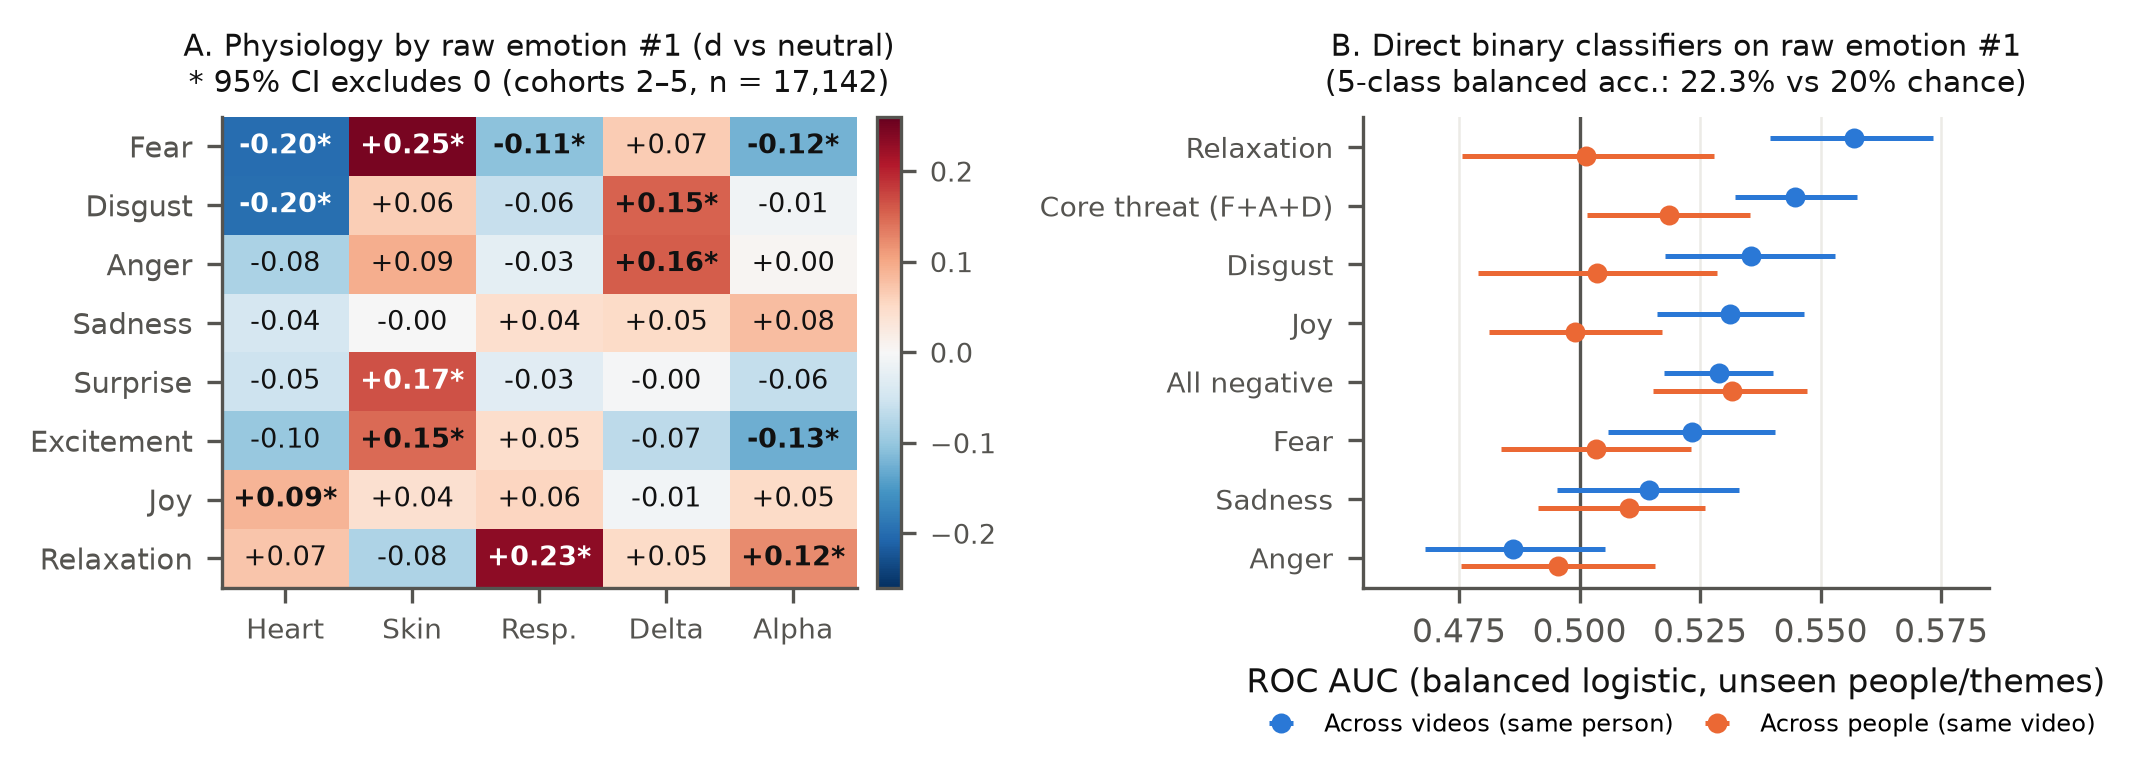
\includegraphics[width=\linewidth]{fig2_emotions.png}
\caption{\textbf{Physiological signatures and direct classifiers on raw rank-1 emotions (Q1).} \textbf{A.} Within-person Cohen's $d$ vs.\ \emph{neutral} (cohorts~2--5): fear combines bradycardia, skin rise, shallow breathing, and alpha drop; disgust is vagal/delta; sadness is flat. \textbf{B.} Balanced binary classifier AUCs across videos within person (blue) and across viewers of the same video (orange).}
\label{fig:emotions}
\end{figure}

Class-balanced binary models trained directly on rank-1 labels (Figure~\ref{fig:emotions}B) confirm no hidden easily decodable subgroup on unseen themes: \emph{relaxation} reaches 0.557 [0.540, 0.573], \emph{core threat} (fear+anger+disgust) 0.545 [0.532, 0.558] (0.550 vs.\ neutral; 0.519 same-video), \emph{disgust} 0.536, \emph{joy} 0.531, \emph{all negative} 0.529 (\textbf{0.532 [0.515, 0.547] same-video}, with a reliably non-zero own heart coefficient $\beta_{\text{own}} = -0.032$ [$-0.049, -0.014$]), \emph{fear} 0.523, \emph{sadness} 0.515, and \emph{anger} 0.486. The unified 5-class classifier (\emph{fear, anger, disgust, sadness, other}) scores 22.3\% balanced accuracy vs.\ 20.0\% chance (OvR AUCs: disgust 0.530, sadness 0.525, fear 0.523, other 0.522, anger 0.502).

In \textbf{unsupervised analysis} (zero labels), PCA on the 36 person-centered physiological variables is dominated by broadband theta/beta EEG (PC1: 44.4\% variance), gamma (PC2: 10.2\%), and parieto-occipital alpha (PC3: 8.3\%, correlating with arousal $r = -0.060$ and valence $+0.052$); only PC4 captures a cardiorespiratory axis weakly correlated with stress ($r = -0.054$). Neither $k$-means ($k = 2$--$6$) nor GMM ($k = 2$--$5$) recovers stress ($\mathrm{ARI} \in [-0.006, +0.008]$, $\mathrm{NMI} \le 0.0006$; stress rates across 4 clusters span 23.1--26.6\%) or 5-class emotions ($\mathrm{NMI} \le 0.0015$), whereas mutual information with video identity is $>10\times$ higher ($\mathrm{NMI} = 0.009$--$0.013$). Spontaneous physiological variance is thus dominated by non-affective EEG fluctuations and stimuli, making supervised or controlled-contrast framing essential.

\subsection{Temporal Sequence, ECG P-QRS-T Morphology, and Rich EEG Dynamics (Q2)}

\paragraph{Second-by-second onset sequence and dimensional controls.}
At 1-s resolution (Figure~\ref{fig:curves}), brain and body move in a fixed order: slow EEG ($\delta$) rises within the first second ($d = +0.11$ to $+0.14$), heart rate drops from 1~s (peaking at $-0.12$ around 7~s), breathing becomes shallower across 2--6~s, and skin conductance rises from 4~s onward (replicated in 52 held-out people with identical onset latency, $d$ up to $+0.25$) \cite{bradley2009,benedek2010}. Control contrasts confirm that heart rate and breathing track unpleasantness (vs.\ arousal-matched excitement: heart $-0.075$, respiration $-0.078$; vs.\ calm negative: $+0.001$ and $-0.009$), whereas skin conductance tracks intensity (vs.\ calm negative $+0.13$, vs.\ excitement null) \cite{lang1993}. For ultra-short HRV, 10-s heart rate agrees closely with 60-s HR ($r = 0.94$, limits $\pm 7.3$~bpm), whereas 10-s RMSSD does not ($r = 0.75$ overall, only $0.43$ within recording; 5-s early-vs-late reliability $r_{\text{within}} = 0.22$), ruling out trial-level RMSSD on brief clips \cite{munoz2015}.

\begin{figure}[t]
\centering
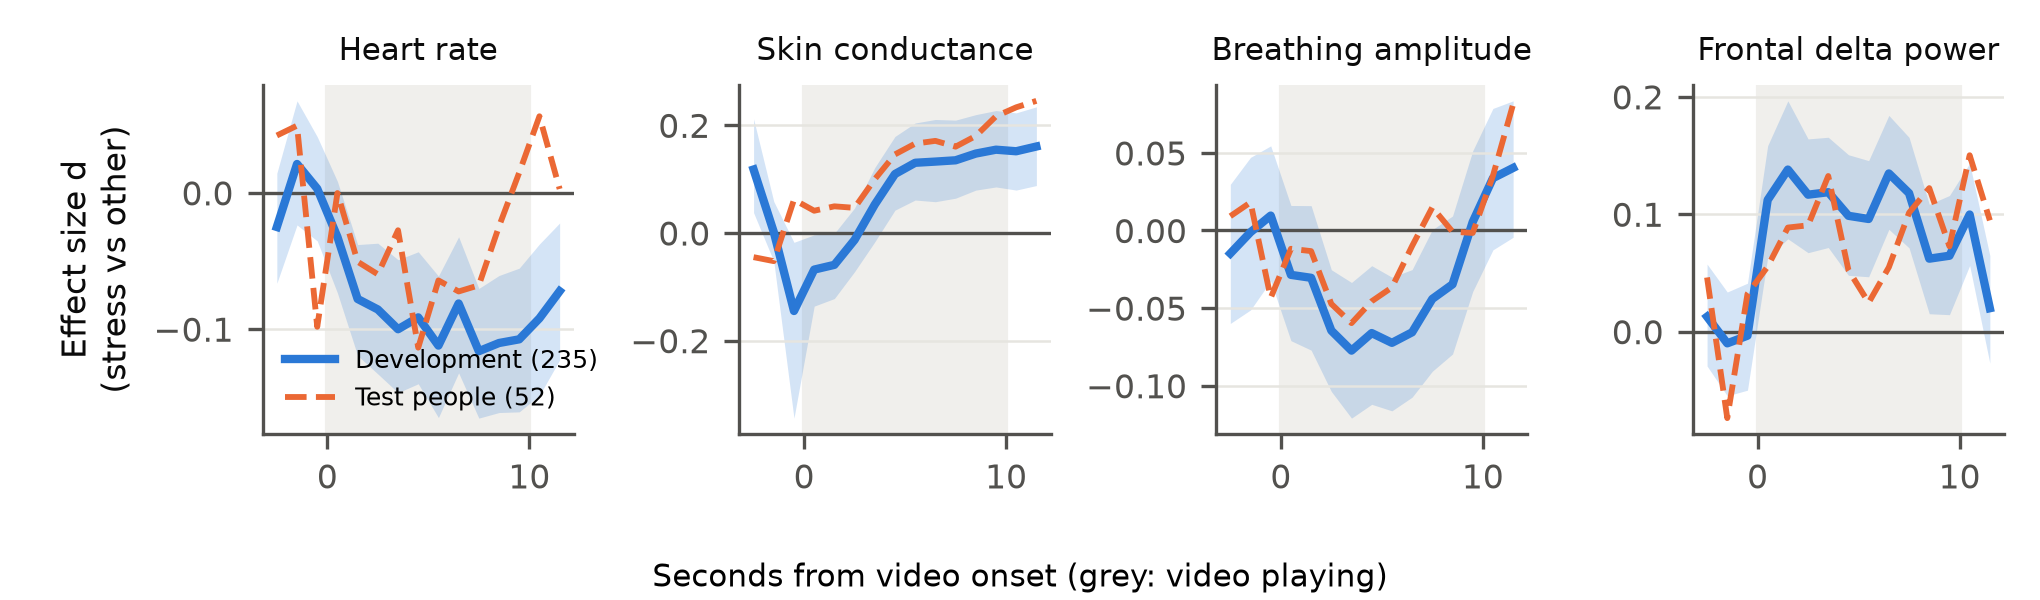
\includegraphics[width=0.96\linewidth]{curves.png}
\caption{\textbf{Second-by-second onset sequence of the four primary physiological responses (Q2).} Within-person effect size (stress vs.\ other trials) relative to the 3-s pre-stimulus baseline. Blue: development (235 people, 95\% CI band). Dashed orange: replication on 52 held-out people.}
\label{fig:curves}
\end{figure}

\paragraph{ECG P-QRS-T morphology: direct electrophysiological proof of vagal braking without PR shortening.}
Our beat-by-beat delineator (after auto-correcting inverted polarity in 96.6\% of trials) achieves 94.7--98.7\% coverage across 22,974 trials with textbook physiological medians: HR 76.3~bpm, RR 786.3~ms, PR peak 128.3~ms, clinical PR interval 134.9~ms, PR segment 39.9~ms, QRS 76.2~ms, QT 360.2~ms, Bazett QTc 402.7~ms, Fridericia QTc 386.9~ms, RT peak 250.2~ms, and T/R ratio 0.53. Across 5-s early vs.\ late phases, within-person reliability of morphological intervals (RT peak $r = 0.71$, QT $0.62$, T/R $0.60$, PR peak $0.49$, clinical PR $0.45$) is two to three times higher than RMSSD ($0.22$).

The primary cardiac electrophysiology result (Figure~\ref{fig:ecg_eeg}A) is crystal clear:
\begin{itemize}
\item \textbf{RR lengthens reliably} ($d = +0.116$ [$+0.071, +0.163$], $+5.06$~ms; early $+0.092$, late $+0.115$, post $+0.058$; vs.\ excitement $+0.126$, vs.\ relaxed $+0.167$).
\item \textbf{PR interval and PR segment (AV-node conduction) are strictly null:} PR peak $d = -0.002$ [$-0.043, +0.036$] ($-0.05$~ms), clinical PR $+0.010$ [$-0.035, +0.053$] ($+0.06$~ms), pure PR segment $-0.005$ [$-0.050, +0.040$] ($-0.04$~ms). Adjusting for $\Delta\mathrm{RR}$ reveals no hidden effect ($-0.001$ to $-0.014$), and both shared and own couplings with valence/arousal sit at zero ($\pm 0.01$). QRS width ($+0.007$) and T/R amplitude ($+0.025$) are likewise null.
\item \textbf{Cardiology QTc artifact:} raw RT peak ($+0.068$ [$+0.027, +0.110$], $+0.22$~ms) and QT ($+0.047$ [$+0.009, +0.085$], $+0.39$~ms) lengthen slightly with bradycardia, making Bazett QTc appear shorter ($d = -0.092$ [$-0.140, -0.045$], $-1.00$~ms; Fridericia $-0.066$). Once $\Delta\mathrm{RR}$ is controlled in within-person regression, \textbf{every QTc/RT/QT shift vanishes completely} (Bazett QTc $-0.007$ [$-0.035, +0.020$], Fridericia $+0.014$, RT peak $+0.011$, QT $+0.034$, all CIs crossing 0)---the classic Bazett over-correction artifact during rapid RR slowing, because ventricular repolarization adapts far more slowly than 10~s.
\end{itemize}
The complete absence of PR shortening (ruling out effects $>0.3$~ms) and T-wave flattening directly proves that 10-s acute cardiac stress reactivity is \textbf{driven by fast vagal (parasympathetic) sinus braking}, not adrenergic acceleration of AV-node conduction.

\begin{figure}[t]
\centering
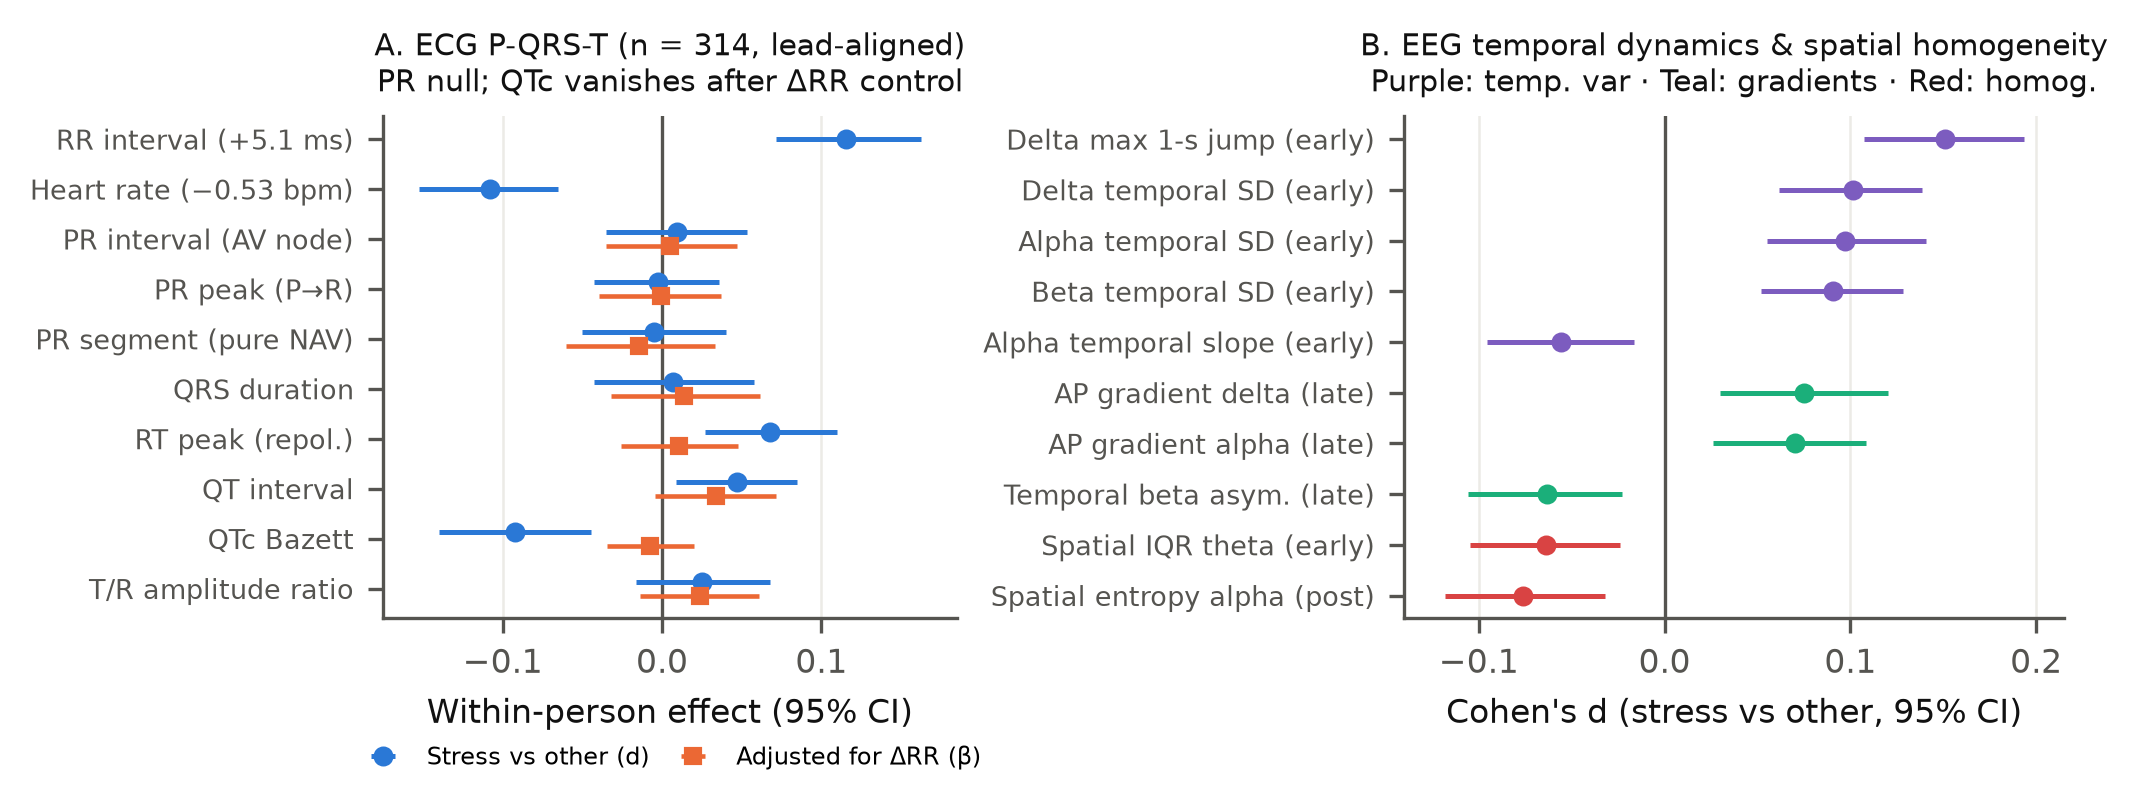
\includegraphics[width=\linewidth]{fig3_ecg_eeg_rich.png}
\caption{\textbf{ECG P-QRS-T morphology and new EEG dynamics (Q2).} \textbf{A.} Within-person 10-s effect sizes (blue) and $\Delta\mathrm{RR}$-adjusted slopes (orange): RR lengthens reliably, PR/QRS/T-amp are strictly null, and apparent QTc shortening vanishes completely after controlling $\Delta\mathrm{RR}$. \textbf{B.} Strong effects in new EEG descriptors: early temporal volatility (purple, up to $d = +0.151$), anterior--posterior gradients and temporal beta asymmetry (green), and biphasic spatial homogeneity (red).}
\label{fig:ecg_eeg}
\end{figure}

\paragraph{EEG temporal volatility and biphasic spatial reorganization.}
Unlike PR waves, the newly proposed EEG features reveal robust effects (Figure~\ref{fig:ecg_eeg}B):
\begin{itemize}
\item \textbf{Broad early temporal volatility ($[0, 5]$~s):} 1-s temporal SD increases across all five bands ($\delta$: $+0.101$ [$+0.061, +0.139$]; $\alpha$: $+0.097$; $\theta$: $+0.096$; $\beta$: $+0.091$; $\gamma$: $+0.057$), while the maximum 1-s delta jump reaches \textbf{$d = +0.151$ [$+0.107, +0.193$]}, matching the strongest static features. Early slopes are negative in alpha ($-0.056$) and theta ($-0.051$), indexing progressive desynchronization across the first 5~s.
\item \textbf{Biphasic spatial reorganization:} during the \emph{early} phase ($[0, 5]$~s), inter-channel dispersion (\texttt{sp\_iqr}) \textbf{decreases} ($\theta$: $-0.064$ [$-0.105, -0.024$], $\delta$: $-0.048$, $\gamma$: $-0.047$), indicating transient spatial homogenization at stimulus onset. In \emph{late} ($[5, 10]$~s) and \emph{post-exposure} ($[10, 12]$~s) phases, this reverses: normalized spatial entropy (\texttt{sp\_ent}) \textbf{drops} ($\alpha$ post: $-0.076$ [$-0.118, -0.032$], $\theta$ post: $-0.062$, $\delta$ post: $-0.058$) while inter-channel SD rises ($+0.055$ to $+0.057$), marking persistent post-clip spatial focalization.
\item \textbf{Gradients and asymmetries:} anterior--posterior gradient (frontal $-$ occipital) shifts strongly anteriorly in the late phase ($\delta$: $+0.075$, $\alpha$: $+0.070$, $\theta$: $+0.065$), combining occipital alpha desynchronization with frontal slow-wave engagement, while temporal beta asymmetry shifts leftward throughout (early $-0.048$, late $-0.063$, post $-0.059$).
\end{itemize}

\subsection{Brain--Heart Coupling (HEP): ICA Did Not Destroy a Hidden Effect (Q3)}

Figure~\ref{fig:hep_raw} directly settles the preprocessing objection. Across the exact same 287 eligible participants (98.6\% coverage, median 13 beats/video in both pipelines, identical R peaks and 62-channel CAR montage):
\begin{itemize}
\item On \texttt{PREPROCESSED} EEG (ICA-cleaned, 100\,$\mu$V), the primary stress effect in 250--600~ms (frontal + central) is not established: $d = +0.039$ [$-0.002, +0.078$] (ECG+RR adjusted: $+0.039$ [$-0.002, +0.081$]).
\item On \textbf{raw \texttt{CURATED} EEG (62-channel CAR, NO ICA, 100\,$\mu$V)}, the result matches \textbf{to the third decimal place}: $d = +0.038$ [$-0.001, +0.077$] (ECG+RR adjusted: $+0.033$ [$-0.006, +0.073$]; 200\,$\mu$V threshold: $+0.006$ [$-0.034, +0.047$]; change vs.\ 3-s pre-stimulus: $-0.010$).
\item The \textbf{exact ICA-removed signal} ($\mathrm{CURATED} - \mathrm{PREPROCESSED}$, locked to identical R peaks) carries zero stress modulation ($d = +0.012$ [$-0.028, +0.053$]) and zero within-person correlation with the 250--600~ms ECG field ($r = -0.004$ [$-0.021, +0.014$]).
\item Only on the extreme \emph{stress vs.\ relaxed} contrast does a tiny positive shift emerge, \textbf{identically} with ICA ($d = +0.072$ [$+0.014, +0.132$]) and without ICA ($d = +0.076$ [$+0.021, +0.137$]).
\end{itemize}
ICA preprocessing therefore did not erase a cardiac-covariant cortical signal: on 10-s clips ($\approx 13$ heartbeats per trial, vs.\ 100--300 beats in resting consciousness studies \cite{park2014,candia2021}), acute stress HEP modulation is at most very small ($|d| < 0.08$).

\begin{figure}[t]
\centering
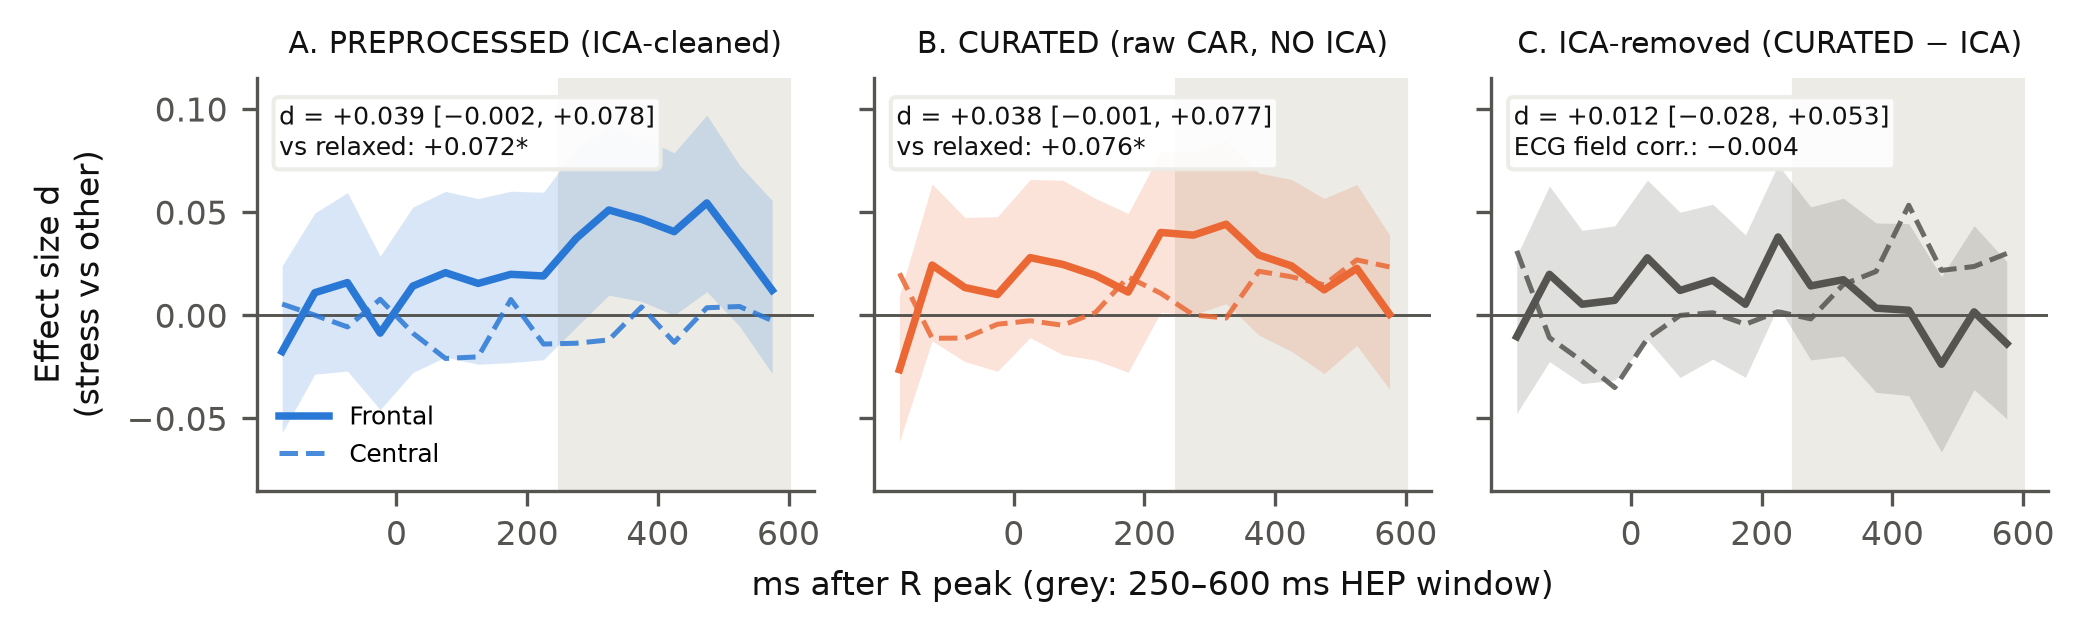
\includegraphics[width=\linewidth]{fig4_hep_raw_vs_ica.png}
\caption{\textbf{Empirical preprocessing control for the heartbeat-evoked potential (Q3).} Stress vs.\ other effect size (287 people; frontal solid + 95\% CI band, central dashed) on identical R peaks and 62 channels: \textbf{A.} \texttt{PREPROCESSED} (ICA). \textbf{B.} Raw \texttt{CURATED} (NO ICA). \textbf{C.} Exact ICA-removed difference ($\text{Raw} - \text{ICA}$). Curves A and B are virtually identical and the ICA-removed waveform is flat.}
\label{fig:hep_raw}
\end{figure}

\subsection{Normative Consensus vs.\ Fixed-Video Appraisal: A Threshold Mechanism (Q4)}

\paragraph{Why the initial linear analysis underestimated subjective appraisal.}
Auditing the 252 videos (Figure~\ref{fig:fixed_video}C) immediately resolves Study~06's apparent paradox (where linear $\beta_{\text{own}}$ of heart rate on valence was 0.004 and diluted same-video AUC was 0.517). Per-video stress rates are strongly skewed: 123 videos sit below 10\%, 112 are polarizing (20--80\%), and 4 exceed 80\%. On high-consensus stressful videos ($p_{v,-i} \ge 50\%$, $n = 5,069$ trials), 63.9\% of viewers are classified \emph{stressed} ($n = 3,241$) and \textbf{33.6\% are borderline} ($n = 1,704$, e.g., unpleasant valence at moderate arousal); only \textbf{2.5\% ($n = 124$, including $n = 63$ very calm) remain genuinely calm ($V \ge 5, A \le 5$)}. Comparing ``stressed'' against ``all other'' viewers of stressful clips was thus comparing stressed against already-negative/borderline viewers 93\% of the time, heavily diluting appraisal effects.

\begin{figure}[t]
\centering
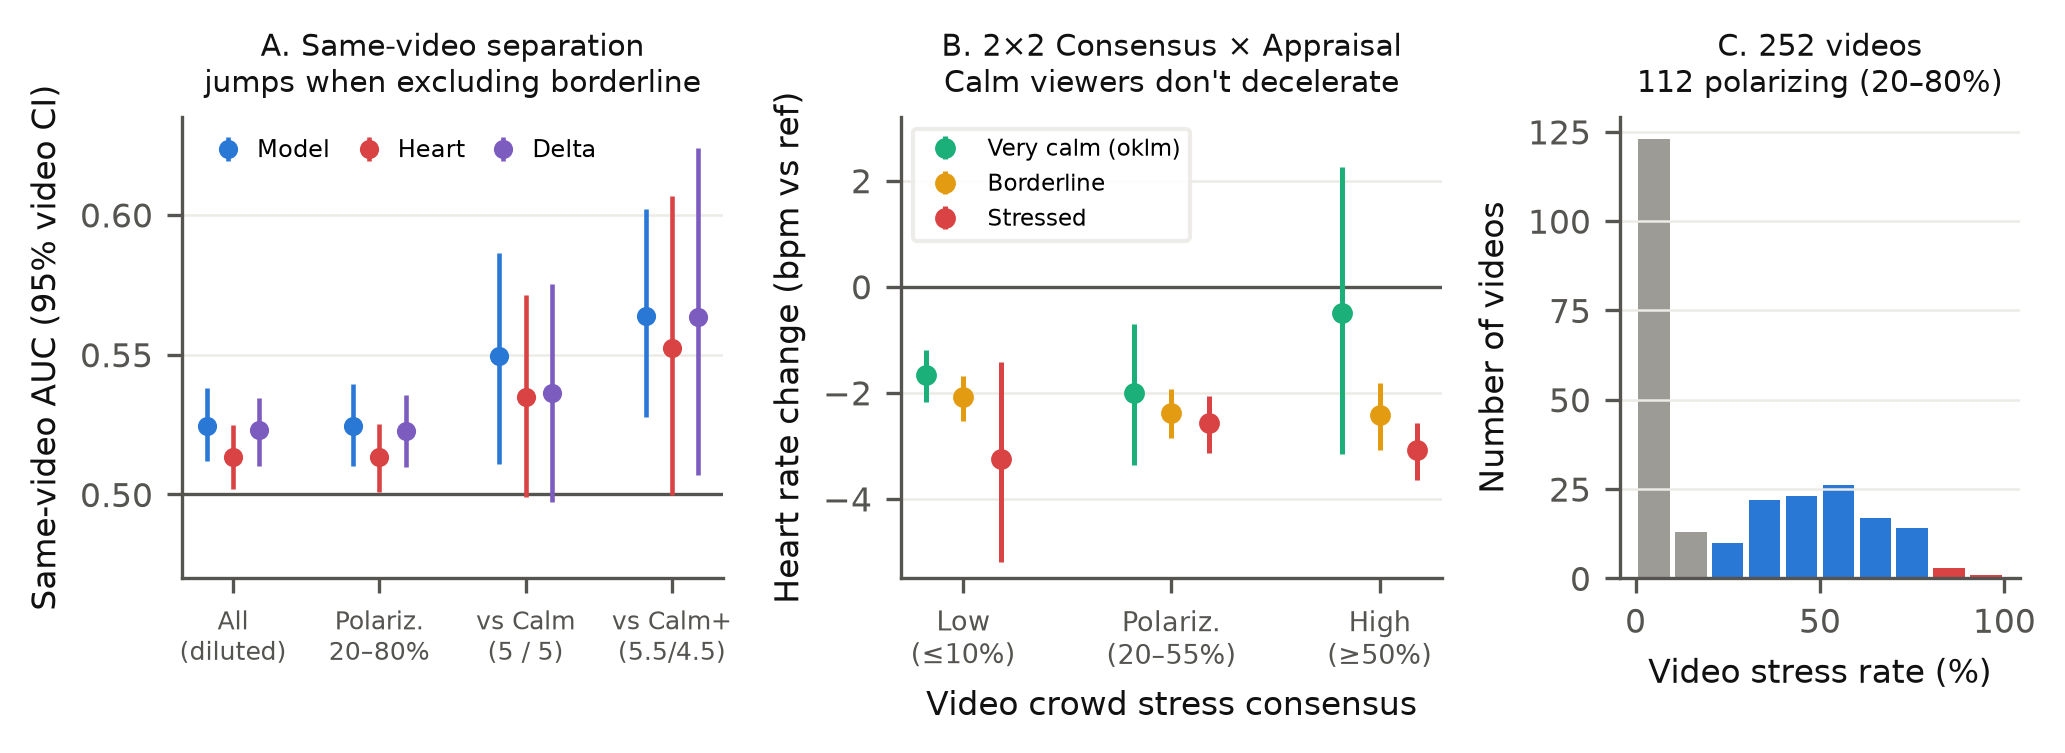
\includegraphics[width=\linewidth]{fig5_fixed_video.png}
\caption{\textbf{Fixed-video appraisal separation and $2\times 2$ Consensus $\times$ Appraisal matrix (Q4).} \textbf{A.} Same-video AUC jumps from 0.525 (diluted) to 0.564 [0.528, 0.602] (heart 0.553, delta 0.564) once stressed viewers are contrasted against genuinely calm viewers of the \emph{same} video. \textbf{B.} Heart-rate change in the $2\times 2$ matrix: on high-consensus stressful clips, calm viewers (teal) do not decelerate ($-0.49$~bpm), unlike borderline ($-2.43$) and stressed ($-3.08$) viewers. \textbf{C.} Stress-rate distribution across all 252 clips.}
\label{fig:fixed_video}
\end{figure}

\paragraph{Non-adjacent fixed-video contrasts and the $2\times 2$ matrix.}
Removing borderline dilution qualitatively changes the conclusion (Figure~\ref{fig:fixed_video}A--B, Table~\ref{tab:matrix2x2}):
\begin{itemize}
\item \textbf{``Stressed vs.\ very calm'' at strictly fixed video} (48 videos, 6,403 pairs): multimodal same-video AUC jumps from 0.525 [0.512, 0.538] (0.524 on polarizing clips) to \textbf{0.564 [0.528, 0.602]}, heart AUC from 0.513 to \textbf{0.553}, delta AUC from 0.523 to \textbf{0.564}, and within-video skin $d$ doubles from $+0.093$ to \textbf{$+0.197$} ($+0.175$ [$+0.019, +0.320$] vs.\ $5/5$ calm across 72 videos). Pure single-axis contrasts at fixed video confirm that skin ($d = +0.072$) and delta ($+0.061$) track pure arousal, while delta ($+0.103$) and the multimodal score (0.534) track pure valence.
\item \textbf{$2\times 2$ Consensus $\times$ Appraisal matrix (Table~\ref{tab:matrix2x2}):} on high-consensus stressful clips ($p_{v,-i} \ge 50\%$), genuinely calm viewers ($V \ge 5.5, A \le 4.5$) show \textbf{zero cardiac deceleration} ($-0.49$~bpm [$-3.16, +2.25$]), \textbf{zero skin-conductance rise} ($+0.014\,\mu$S, identical to calm viewers on neutral clips $+0.014\,\mu$S), and no delta rise ($-0.073$), whereas stressed viewers on those exact same clips show $-3.08$~bpm, $+0.041\,\mu$S, and $+0.021$. Conversely, when viewers feel stressed on low-consensus neutral clips ($p_{v,-i} \le 10\%$, $n = 113$), heart rate drops $-3.24$~bpm [$-5.19, -1.43$] and skin jumps $+0.071\,\mu$S [$+0.022, +0.136$].
\item \textbf{Paired within-person contrasts:} among people who experienced some high-consensus stressful clips as calm and others as stressed ($N = 26$), the pure appraisal effect reaches \textbf{$-2.97$~bpm [$-4.81, -1.10$] ($d = -0.41$ [$-0.65, -0.13$])} for heart rate, \textbf{$+0.033\,\mu$S [$+0.003, +0.066$] ($d = +0.31$)} for skin, and \textbf{$d = +0.45$ [$+0.00, +0.95$]} for delta (on polarizing clips $N = 36$--$60$: skin $d = +0.26$, delta $d = +0.27$ to $+0.47$, heart $-1.72$~bpm). Conversely, holding viewer state calm while varying stimulus consensus (pure stimulus effect in calm viewers, $N = 29$), \textbf{only alpha desynchronization fires automatically} ($d = -0.33$ [$-0.56, -0.12$]; $-0.41$ in very calm viewers), whereas skin ($-0.06$), respiration ($-0.04$), delta ($-0.13$), and bradycardia do not trigger.
\end{itemize}

\begin{table}[t]
\centering\footnotesize
\setlength{\tabcolsep}{4.5pt}
\begin{tabular}{@{}llrrrrr@{}}
\toprule
Video consensus ($p_{v,-i}$) & Viewer state & Trials & Heart (bpm) & Skin ($\mu$S) & Resp. & Delta ($\log_{10}$)\\
\midrule
Low ($\le 10\%$) & Very calm ($V\ge 5.5, A\le 4.5$) & 4,414 & $-1.67$ [$-2.17, -1.19$] & $+0.014$ & $-0.092$ & $-0.040$\\
 & Borderline & 5,831 & $-2.08$ [$-2.53, -1.68$] & $+0.025$ & $-0.156$ & $-0.049$\\
 & Stressed ($V\le 4, A\ge 6$) & 113 & $\mathbf{-3.24}$ [$-5.19, -1.43$] & $\mathbf{+0.071}$ & $-0.236$ & $-0.059$\\
\midrule
Polarizing (20--55\%) & Very calm & 167 & $-2.00$ [$-3.35, -0.71$] & $+0.021$ & $-0.197$ & $-0.094$\\
 & Borderline & 3,578 & $-2.39$ [$-2.85, -1.94$] & $+0.032$ & $-0.176$ & $-0.028$\\
 & Stressed & 2,855 & $-2.58$ [$-3.14, -2.06$] & $\mathbf{+0.049}$ & $-0.188$ & $\mathbf{+0.009}$\\
\midrule
High ($\ge 50\%$) & Very calm (unperturbed) & 63 & $\mathbf{-0.49}$ [$-3.16, +2.25$] & $\mathbf{+0.014}$ & $-0.111$ & $-0.073$\\
 & Borderline & 1,704 & $-2.43$ [$-3.08, -1.81$] & $+0.029$ & $-0.181$ & $-0.002$\\
 & Stressed & 3,241 & $\mathbf{-3.08}$ [$-3.64, -2.57$] & $\mathbf{+0.041}$ & $-0.203$ & $\mathbf{+0.021}$\\
\bottomrule
\end{tabular}
\caption{$2\times 2$ Stimulus Consensus $\times$ Viewer Appraisal matrix (raw mean changes from the 3-s pre-stimulus baseline, averaged across participants with 95\% bootstrap CIs).}
\label{tab:matrix2x2}
\end{table}

\paragraph{Nonlinear threshold structure of dose--response curves.}
Person-centered 8-bin dose--response curves cleanly explain how a near-zero linear $\beta_{\text{own}}$ coexists with a clear appraisal effect (consistent with shared autonomic synchronization during film viewing \cite{golland2014} and modest linear coherence between experience and physiology \cite{mauss2005}):
\begin{itemize}
\item Across \textbf{valence}, heart rate behaves as an \textbf{all-or-nothing step function at valence = 5}: flat and negative across the entire unpleasant half ($[1, 2)$: $-0.42$~bpm, $[2, 3)$: $-0.35$, $[3, 4)$: $-0.25$, $[4, 5)$: $-0.20$), jumping sharply positive above 5 ($+0.52$ on $[5, 6)$, $+0.54$ on $[8, 9]$). Once a clip is judged unpleasant, bradycardia scarcely scales with finer gradations of unpleasantness---explaining the flat linear slope within unpleasant videos.
\item Across \textbf{arousal}, heart rate traces a \textbf{non-monotonic U-curve}: flat up to 5 ($+0.02$ to $+0.16$~bpm), reaching peak bradycardia on $[6, 7)$ ($-0.55$~bpm), then \textbf{rebounding} on $[7, 8)$ ($+0.05$~bpm) and $[8, 9]$ ($+0.13$~bpm) as sympathetic drive engages. Conversely, skin conductance and delta act as \textbf{high-threshold alarms}: flat across 1--7 (skin $-0.012$ to $-0.004\,\mu$S), firing steeply only on $[7, 8)$ ($+0.014\,\mu$S, delta $+0.016$) and $[8, 9]$ ($+0.032\,\mu$S, delta $+0.036$).
\end{itemize}

\subsection{EEG Topography of Stress Sensitivity and Anxiety Correlates (Q5)}

\paragraph{Trial-level idiosyncratic sensitivity ($\beta_{\text{own}}$) and pre-ICA ocular control.}
Mapping all 6 regions $\times$ 5 bands (Figure~\ref{fig:sens_models}A) uncovers a well-structured spectral topography of individual sensitivity to negative valence beyond video consensus:
\begin{itemize}
\item \textbf{Prefrontal fast $\beta/\gamma$ rhythms:} the strongest own-rating slopes on the scalp appear in \textbf{frontal gamma} ($\beta_{\text{own}} = -0.039$ [$-0.056, -0.022$]) and \textbf{frontal beta} ($-0.035$ [$-0.053, -0.017$]), alongside left-temporal gamma for own arousal ($+0.030$ [$+0.013, +0.047$]). Across 62 electrodes, own beta peaks bilaterally over prefrontal sites (Fp2 $-0.034$, Fp1 $-0.033$, AF7 $-0.029$, F4 $-0.028$, AF8 $-0.028$, F3 $-0.027$).
\item \textbf{Genuinely cortical centroparietal delta:} delta tracks own valence across all six regions (peaking in \textbf{central} $-0.037$ [$-0.053, -0.020$] and right temporal $-0.030$), with electrode maxima at \textbf{FC3 ($-0.041$), POz ($-0.041$), Pz ($-0.040$), and C3 ($-0.038$)}---not frontopolar sites. Controlling for the pre-ICA Fp1/Fp2 ocular peak-to-peak proxy (strongly correlated with overall delta, $\beta = +0.416$) confirms that the blink proxy itself has zero own arousal coupling ($\beta_{\text{own}} = +0.0004$ [$-0.017, +0.018$]) and leaves \textbf{93\% of delta's own coupling intact} ($+0.0286 \to +0.0267$ [$+0.0102, +0.0423$]), resolving Study~06's ocular caveat.
\item \textbf{Alpha, theta, and frontal alpha asymmetry (FAA):} $\beta_{\text{own}}$ is null for alpha and theta in every region, and FAA shows zero effect in any band (alpha FAA $d = +0.021$ [$-0.023, +0.064$]), consistent with the null meta-analysis of van der Vinne et al.\ \cite{vandervinne2017}.
\end{itemize}

\paragraph{Between-subject correlates of trait stress sensitivity ($N = 314$).}
Participants vary widely in their propensity to rate the same videos as more stressful than peers (raw stress rate IQR 15.1--32.7\%; consensus-adjusted bias SD 12.1 percentage points). Adjusted for cohort, higher trait stress/arousal sensitivity correlates with: (i)~\textbf{higher resting pre-stimulus heart rate} ($r = +0.140$ [$+0.032, +0.244$], $\rho = +0.142$); (ii)~\textbf{higher scalp-wide pre-stimulus gamma power}, maximal in frontal ($r = +0.165$ [$+0.061, +0.279$], $\rho = +0.185$), central ($+0.148$), and occipital ($+0.142$) regions; (iii)~\textbf{lower pre-stimulus temporal theta} (right temporal $r = -0.149$ [$-0.260, -0.033$], left temporal $-0.126$); and (iv)~female sex ($r = +0.172$ for stress bias, $+0.226$ for negative valence, replicating classic affective sex differences \cite{bradley2001}). Crucially, subjectively sensitive individuals do \emph{not} display larger phasic autonomic responses (non-significant trend toward smaller skin response, $r = -0.11$). This profile---elevated basal heart rate, tonic and phasic prefrontal gamma hyper-activity, and null FAA---closely parallels neurobiological models of anxious hypervigilance \cite{oathes2008}, while warranting caution regarding potential residual prefrontal/temporal micro-EMG in gamma even after ICA.

\subsection{Benchmark of 4 Phases, \texorpdfstring{$\Delta(t\to t+1)$}{Delta(t->t+1)} Transitions, and Sequence Architectures (Q6)}
\label{sec:seq_results}

Benchmarking all twelve configurations on the fresh person $\times$ theme split (development: 12,052 trials, 249 people, 60 themes; sealed tests: 1,646 trials on 65 unseen people $\times$ 24 unseen themes, 3,285 on 65 unseen people, 5,991 on 24 unseen themes) clearly validates the temporal-resolution and EEG-feature upgrades while confirming the null predictive value of PR intervals and nonlinear heads on unseen themes (Figure~\ref{fig:sens_models}B, Table~\ref{tab:seq_models}):
\begin{enumerate}
\item \textbf{Replacing 1-s bins with 4 physiological phases delivers the largest efficiency gain:} using \textbf{three times fewer features} ($p = 114$ vs.\ 340), 4-phase logistic regression outperforms the 1-s baseline on every unseen-theme test---development $+0.014$ (0.546 $\to$ 0.560, and $+0.029$ vs.\ excitement), strictest double-unseen sealed test $+0.044$ (0.526 [0.481, 0.570], overlapping chance $\to$ \textbf{0.570 [0.519, 0.618]}), and unseen themes $+0.019$ (0.527 $\to$ 0.546). Averaging over 2--5~s phases sharply denoises heart-rate and EEG spectral estimates.
\item \textbf{Ablations pinpoint what truly helps:} starting from 4 phases + $\Delta(t\to t+1)$ transitions ($p = 190$: dev 0.561, new both 0.565), adding \textbf{ECG P-QRS-T morphology} adds zero gain (dev 0.559, new both 0.562, new themes 0.540), directly echoing Q2's physiological null. By contrast, adding \textbf{EEG temporal volatility} ($+30$ features) yields the largest single-block development jump (0.567 [0.552, 0.582], lifting dev same-video AUC from 0.520 to \textbf{0.539 [0.519, 0.555]}) and pushes new-both to 0.580; adding \textbf{EEG spatial homogeneity and gradients} lifts new-both to \textbf{0.582 [0.531, 0.633]} and achieves the highest unseen-theme same-video AUC (\textbf{0.542 [0.520, 0.562]}).
\item \textbf{Continuous supervision and multi-scale sequence convolutions:} on the full enriched feature set ($p = 448$), linear classification reaches \textbf{0.589 [0.540, 0.635]} on the strictest double-unseen test ($+0.063$ above the 1-s baseline; 0.566 vs.\ excitement), while \textbf{continuous valence--arousal Ridge} (\texttt{enriched\_full\_ridge\_va}) is the \textbf{best overall model}: dev \textbf{0.576 [0.561, 0.591]} ($+0.030$ vs.\ 1-s; 0.602 vs.\ relaxed), new-both \textbf{0.586 [0.536, 0.633]} (0.602 vs.\ calm negative, 0.604 vs.\ relaxed), unseen themes \textbf{0.558 [0.535, 0.581]} (best), and unseen people \textbf{0.607 [0.580, 0.633]} (\textbf{0.656 [0.623, 0.689]} vs.\ relaxed). Applying multi-scale 1D temporal convolutions and $t\to t+1$ derivatives to the 1-s sequence (\texttt{sequence\_multiscale\_conv}, $p = 620$) strongly outperforms flat 1-s bins (dev 0.546 $\to$ \textbf{0.569}, best same-video AUC on dev \textbf{0.541} and on new-both \textbf{0.527}); combining sequence + enriched linearly reaches 0.573 on dev and 0.573 on new-both.
\item \textbf{Ceiling of nonlinear heads on unseen stimuli:} \emph{HistGradientBoosting} excels on seen themes (unseen people 0.608, same-video 0.571, calm negative 0.636) but drops on unseen themes (0.532 vs.\ 0.558 for Ridge), and the MLP on all 1,068 features trails regularized linear heads (dev 0.552, unseen themes 0.531). With 249 training participants and low single-trial SNR, physiological representation quality outweighs classifier nonlinearity.
\end{enumerate}

\begin{figure}[t]
\centering
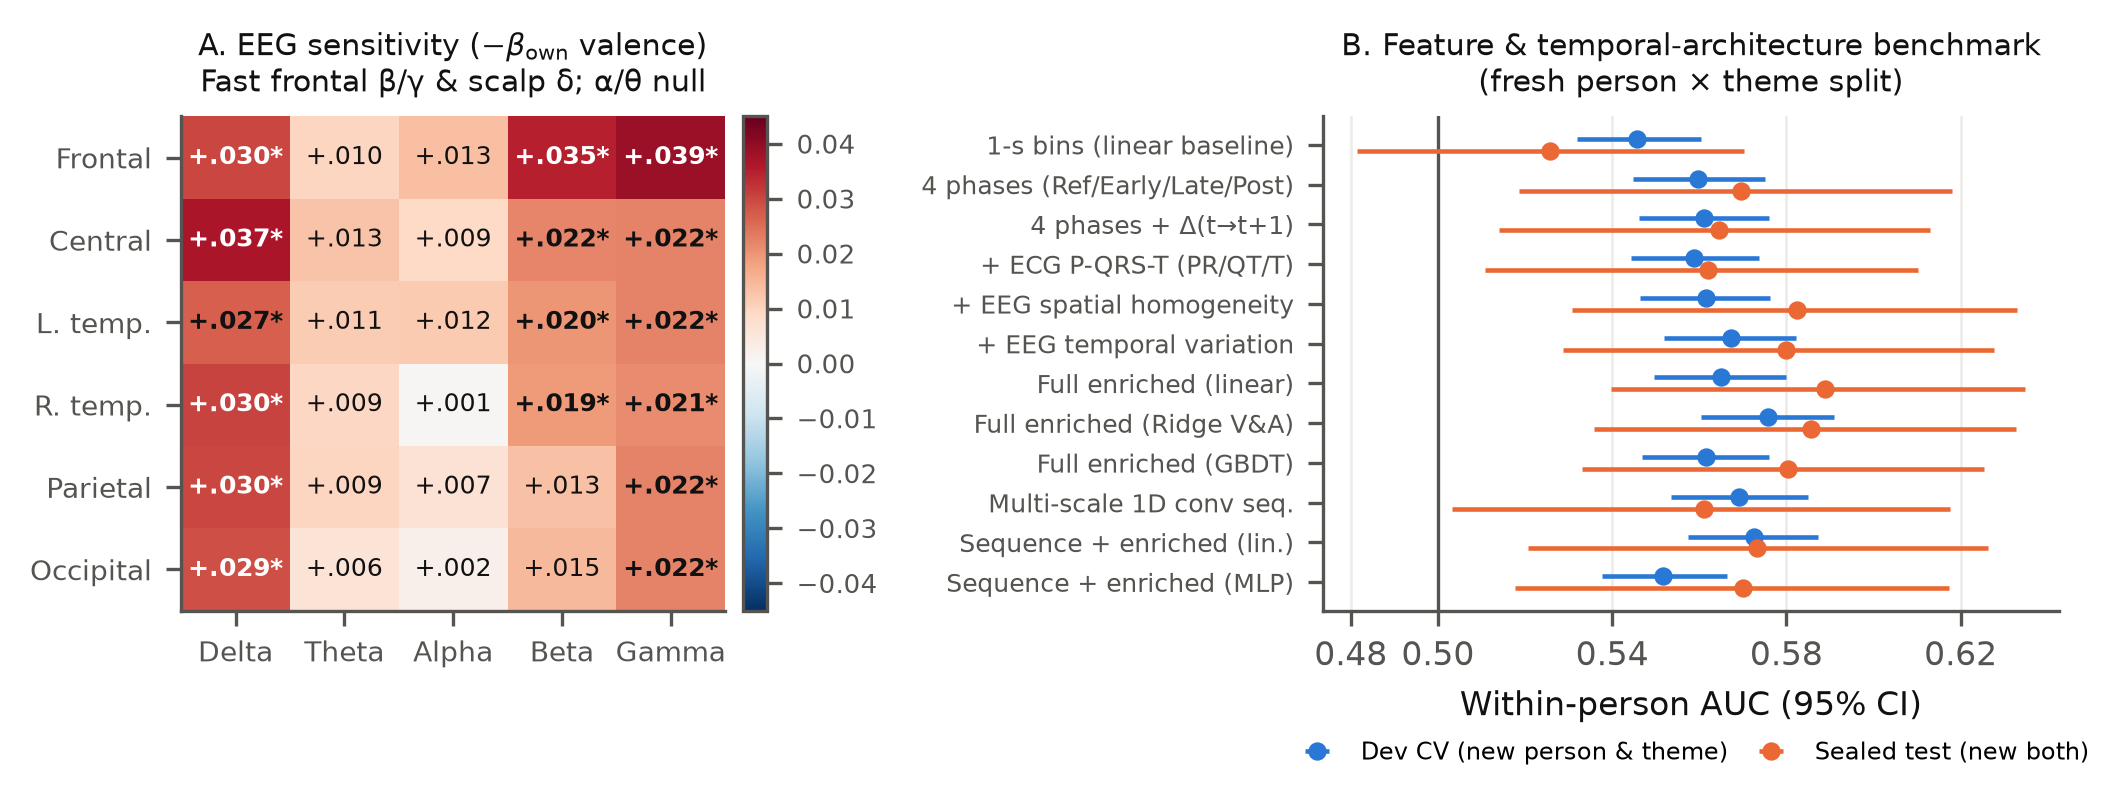
\includegraphics[width=\linewidth]{fig6_sensitivity_models.png}
\caption{\textbf{EEG topography of individual sensitivity (Q5) and benchmark of 12 temporal models (Q6).} \textbf{A.} $6\text{ regions} \times 5\text{ bands}$ map of $-\beta_{\text{own}}$ (valence): individual sensitivity concentrates in frontal $\beta/\gamma$ and scalp-wide $\delta$, while $\alpha/\theta$ are null (*: 95\% CI excludes 0). \textbf{B.} Within-person AUC on the fresh person $\times$ theme split in development (blue) and on the double-unseen sealed test (orange). Enriched 4-phase and sequence representations gain $+0.030$ on dev and up to $+0.063$ on the strict sealed test over flat 1-s bins.}
\label{fig:sens_models}
\end{figure}

\begin{table}[t]
\centering\footnotesize
\begin{tabular}{@{}lrrrrrrr@{}}
\toprule
Configuration & $p$ & Dev WP & Dev SV & New Both & New Ppl & New Thm & vs.\ Rel.\ (P)\\
\midrule
1-s bins (linear baseline) & 340 & 0.546 & 0.519 & 0.526 & 0.600 & 0.527 & 0.632\\
4 phases (Ref/Early/Late/Post) & 114 & 0.560 & 0.524 & 0.570 & 0.599 & 0.546 & 0.632\\
4 phases + $\Delta(t\to t+1)$ & 190 & 0.561 & 0.520 & 0.565 & 0.605 & 0.548 & 0.650\\
\quad $+$ ECG P-QRS-T (PR/QT/T) & 243 & 0.559 & 0.523 & 0.562 & 0.608 & 0.540 & 0.649\\
\quad $+$ EEG spatial homogeneity & 365 & 0.562 & 0.521 & 0.582 & 0.600 & 0.555 & 0.640\\
\quad $+$ EEG temporal variation & 220 & 0.567 & 0.539 & 0.580 & 0.599 & 0.547 & 0.640\\
Full enriched (linear) & 448 & 0.565 & 0.533 & \textbf{0.589} & 0.602 & 0.552 & 0.643\\
Full enriched (Ridge V\&A) & 448 & \textbf{0.576} & 0.527 & 0.586 & 0.607 & \textbf{0.558} & \textbf{0.656}\\
Full enriched (GBDT) & 448 & 0.562 & 0.514 & 0.580 & \textbf{0.608} & 0.532 & 0.644\\
Multi-scale 1D conv sequence & 620 & 0.569 & \textbf{0.541} & 0.561 & 0.607 & 0.540 & 0.639\\
Sequence + enriched (linear) & 1,068 & 0.573 & 0.539 & 0.573 & 0.607 & 0.549 & 0.654\\
Sequence + enriched (MLP) & 1,068 & 0.552 & 0.527 & 0.570 & 0.608 & 0.531 & 0.648\\
\bottomrule
\end{tabular}
\caption{Full benchmark of twelve feature representations and architectures on the fresh person $\times$ theme split (\texttt{habs-revision-2026-11-23}). WP: within-person AUC; SV: pair-weighted same-video AUC; New Both: sealed unseen people $\times$ unseen themes (65 $\times$ 24); New Ppl: 65 unseen people; New Thm: 24 unseen themes; vs.\ Rel.\ (P): stress vs.\ relaxed on unseen people.}
\label{tab:seq_models}
\end{table}

\section{Discussion and Outlook}

\begin{table}[t]
\centering\small
\begin{tabularx}{\linewidth}{@{}l X l@{}}
\toprule
Question & Main finding & Key figure\\
\midrule
Q1, criterion & Purity validated on raw emotions; autonomic divergence & 89.2\% rank 1 (97.2\% ranks 1--3); opt.\ $3/7$\\
Q1, emotions & Fear (HR+SC+$\alpha$), disgust (HR+$\delta$), sadness flat; unsup.\ null & Fear SC $+0.25$, HR $-0.20$; $\mathrm{ARI} < 0.009$\\
Q2, ECG P-QRS-T & RR lengthens, PR (AV node) strictly null, QTc = Bazett artifact & RR $+5.1$~ms; PR $-0.05$~ms; QTc ctrl $-0.007$\\
Q2, rich EEG & Strong early temporal volatility; biphasic spatial shift & $\delta$ jump $+0.151$; post $\alpha$ entropy $-0.076$\\
Q3, raw/ICA HEP & ICA does not destroy HEP; primary effect null in both & Raw $+0.038$ vs.\ ICA $+0.039$; diff.\ $+0.012$\\
Q4, fixed video & Non-adjacent contrast (vs.\ calm) unlocks appraisal effect & AUC 0.564; $2\times 2$ HR $-2.97$~bpm ($d = -0.41$)\\
Q5, sensitivity & Frontal $\beta/\gamma$ + centroparietal $\delta$ (survives ocular proxy) & Frontal $\gamma$ $-0.039$; trait HR $+0.14$, $\gamma$ $+0.17$\\
Q6, 4 ph.\ \& seq. & 4 phases + rich EEG + Ridge V\&A / 1D conv beat 1-s; PR/MLP null & New Both 0.526 $\to$ 0.589; Ridge dev 0.576, rel.\ 0.656\\
\bottomrule
\end{tabularx}
\caption{Summary of the six research questions and verified empirical findings across 314 participants.}
\label{tab:summary}
\end{table}

\paragraph{A three-branch neurophysiological model of brief acute stress.}
Together (Table~\ref{tab:summary}), these results define a coherent three-branch physiological architecture during brief aversive exposure:
\begin{enumerate}
\item \textbf{An automatic, stimulus-driven attentional branch:} parieto-occipital alpha desynchronization occurs even when a viewer stays completely calm during a stressful clip ($d = -0.33$ to $-0.41$) and exhibits zero own-appraisal coupling.
\item \textbf{An appraisal-gated vagal orienting branch (threshold mechanism):} once a stimulus crosses the subjective aversiveness threshold ($V < 5$), heart rate decelerates (from 1~s, $-2.4$ to $-3.1$~bpm) and breathing becomes shallower (2~s), without PR shortening or T-wave flattening---direct electrophysiological proof of fast parasympathetic sinus braking without pronounced adrenergic AV-node acceleration. When a viewer remains calm during the same stimulus, this bradycardia does not fire ($-0.49$~bpm).
\item \textbf{A high-threshold sympathetic and cortical alarm branch:} once arousal exceeds~7, sudomotor skin conductance (from 4~s) and centroparietal delta power/volatility double, accompanied by prefrontal $\beta/\gamma$ activity scaling with individual sensitivity, while cardiac sympathetic recruitment begins countering vagal bradycardia (U-shaped HR rebound at $A = 8$--$9$).
\end{enumerate}

\paragraph{Implications for non-communicating clinical monitoring and affective research.}
This framework directly informs the design and validation of acute stress or pain monitors in non-verbal populations (neonates and pre-verbal pediatrics, locked-in syndrome, coma, general anesthesia):
\begin{itemize}
\item \textbf{Do not assume linear tachycardia:} brief aversive events first elicit vagal deceleration (U-shaped with arousal), whereas intense somatic nociception or sustained stress recruits sympathetic tachycardia. Monotonic linear HR rules miss this reversal; phased and nonlinear representations are required.
\item \textbf{Caution with ultra-short cardiac metrics:} on 10-s windows, RMSSD is unreliable ($r_{\text{within}} = 0.22$--$0.43$), Bazett QTc produces severe over-correction artifacts during rapid RR shifts, and PR intervals show no measurable adrenergic signal at this timescale. Likewise, HEP requires far more than $\approx 13$ beats per trial.
\item \textbf{A rigorous validation standard:} holding out both people and themes prevents stimulus memorization but does not separate subjective state from sensory input. Conversely, fixed-stimulus controls contrasting ``stressed vs.\ all else'' dilute appraisal with borderline trials. Studies should jointly report: (i)~unseen-person/unseen-stimulus AUC, (ii)~fixed-stimulus AUC and $d$ on \emph{non-adjacent contrasts} (stressed vs.\ calm), and (iii)~the $2\times 2$ Consensus $\times$ Appraisal matrix.
\item \textbf{Single-trial clinical ceiling:} although enriched 4-phase and sequence representations yield a solid $+0.030$ to $+0.063$ AUC gain on the strictest split, single-trial AUC still plateaus around 0.56--0.61 on unseen people/themes (0.65--0.66 vs.\ relaxed). Standalone clinical decisions cannot rely on an isolated 10-s window; multi-episode temporal aggregation, individual resting calibration (basal HR, spectral profile), and validation on active-stress or nociceptive paradigms are essential next steps.
\end{itemize}

\paragraph{Limitations and reproducibility.}
Findings derive from passive 10-s videos in healthy adults: metabolic, social, or acute somatic pain stressors (notably in pediatrics) more strongly recruit adrenergic sympathetic drive (tachycardia and potential PR shortening beyond 10--30~s). The single ECG lead precludes multi-lead vector analysis. Extreme cells of the $2\times 2$ matrix (very calm viewers on high-consensus stressful clips, $n = 63$) have modest counts and wider CIs. Although our pre-ICA ocular proxy rules out blink leakage for centroparietal delta, residual cranial micro-EMG cannot be completely excluded in prefrontal/temporal $\beta/\gamma$. Finally, lack of repeated ratings per video--person pair prevents direct test--retest measurement of self-report reliability. All extraction (\texttt{decoding/rich\_extract.py}), analysis (\texttt{decoding/revision.py}), frozen protocols (\texttt{journal/}), aggregate metrics, and figure scripts (\texttt{docs/research/revision/}) are versioned in the repository; no participant-level data leave HABS servers.

\begin{thebibliography}{99}\footnotesize\setlength{\itemsep}{0.5pt}
\bibitem{giannakakis2015} G. Giannakakis, D. Grigoriadis, M. Tsiknakis. Detection of stress/anxiety state from EEG features during video watching. IEEE EMBC 2015, 6034--6037.
\bibitem{gerster2026} M. Gerster et al. Stimulus identity rather than emotion drives EEG classification on the FACED dataset. bioRxiv 2026, doi:10.64898/2026.06.12.731889.
\bibitem{bradley2001} M. M. Bradley, M. Codispoti, D. Sabatinelli, P. J. Lang. Emotion and motivation II: sex differences in picture processing. Emotion 1 (2001) 300--319.
\bibitem{bradley2009} M. M. Bradley. Natural selective attention: orienting and emotion. Psychophysiology 46 (2009) 1--11.
\bibitem{benedek2010} M. Benedek, C. Kaernbach. A continuous measure of phasic electrodermal activity. J. Neurosci. Methods 190 (2010) 80--91.
\bibitem{lang1993} P. J. Lang, M. K. Greenwald, M. M. Bradley, A. O. Hamm. Looking at pictures: affective, facial, visceral, and behavioral reactions. Psychophysiology 30 (1993) 261--273.
\bibitem{palomba2000} D. Palomba, M. Sarlo, A. Angrilli, A. Mini, L. Stegagno. Cardiac responses associated with affective processing of unpleasant film stimuli. Int. J. Psychophysiol. 36 (2000) 45--57.
\bibitem{hagenaars2014} M. A. Hagenaars, K. Roelofs, J. F. Stins. Human freezing in response to affective films. Anxiety, Stress, \& Coping 27 (2014) 27--37.
\bibitem{schubring2019} D. Schubring, H. T. Schupp. Affective picture processing: alpha- and lower beta-band desynchronization reflects emotional arousal. Psychophysiology 56 (2019) e13386.
\bibitem{siegel2018} E. H. Siegel et al. Emotion fingerprints or emotion populations? A meta-analytic investigation of autonomic features of emotion categories. Psychol. Bull. 144 (2018) 343--393.
\bibitem{mauss2005} I. B. Mauss et al. The tie that binds? Coherence among emotion experience, behavior, and physiology. Emotion 5 (2005) 175--190.
\bibitem{golland2014} Y. Golland, K. Keissar, N. Levit-Binnun. Studying the dynamics of autonomic activity during emotional experience. Psychophysiology 51 (2014) 1101--1111.
\bibitem{park2014} H.-D. Park, S. Correia, A. Ducorps, C. Tallon-Baudry. Spontaneous fluctuations in neural responses to heartbeats predict visual detection. Nat. Neurosci. 17 (2014) 612--618.
\bibitem{candia2021} D. Candia-Rivera et al. Neural responses to heartbeats detect residual signs of consciousness during resting state in postcomatose patients. J. Neurosci. 41 (2021) 5251--5262.
\bibitem{parkblanke2019} H.-D. Park, O. Blanke. Heartbeat-evoked cortical responses: underlying mechanisms, functional roles, and methodological considerations. NeuroImage 197 (2019) 502--511.
\bibitem{munoz2015} M. L. Munoz et al. Validity of (ultra-)short recordings for heart rate variability measurements. PLoS ONE 10 (2015) e0138921.
\bibitem{vandervinne2017} N. van der Vinne et al. Frontal alpha asymmetry as a diagnostic marker in depression: fact or fiction? A meta-analysis. NeuroImage: Clinical 16 (2017) 79--87.
\bibitem{oathes2008} D. J. Oathes, W. J. Ray, A. S. Yamasaki, T. D. Borkovec, L. G. Castonguay, M. G. Newman, J. Nitschke. Worry, generalized anxiety disorder, and emotion: evidence from the EEG gamma band. Biol. Psychol. 79 (2008) 165--170.
\bibitem{varoquaux2018} G. Varoquaux. Cross-validation failure: small sample sizes lead to large error bars. NeuroImage 180 (2018) 68--77.
\end{thebibliography}

\end{document}
